\documentclass[12pt]{article}

% ============ 1. KHAI BÁO TẤT CẢ PACKAGE ============
\usepackage{hcmus-report-template}
% Các gói bổ trợ cho nội dung (Tránh lỗi Undefined control sequence hoặc thiếu định dạng bảng/thuật toán)
\usepackage{amsmath,amssymb}
\usepackage{bm}
\usepackage{booktabs,multirow,array}
\usepackage{graphicx}
\usepackage{caption,subcaption}
\usepackage{float}
\usepackage{xcolor}
\usepackage{algorithm}
\usepackage{algpseudocode}
\usepackage{enumitem}
\usepackage{tabularx}
\usepackage{tikz}
\usetikzlibrary{arrows.meta}
% ============ 2. CẤU HÌNH & TÙY CHỈNH ============
% Disable indentation on new paragraphs
\setlength{\parindent}{0pt}

% Line spacing 1.5
\renewcommand{\baselinestretch}{1.5}

% Cấu hình caption và enumitem
\captionsetup{font=small,labelfont=bf}
\captionsetup[table]{position=top}
\setlist{itemsep=2pt,topsep=3pt}

% Định nghĩa macro toán học và code
\newcommand{\code}[1]{\texttt{#1}}
\DeclareMathOperator*{\argmax}{arg\,max}
\DeclareMathOperator*{\argmin}{arg\,min}
\newcommand{\R}{\mathbb{R}}


% Define course name, report name and report title.
\newcommand{\coursename}{Nhận Dạng Mẫu}
\newcommand{\reportname}{Nhận dạng chữ số viết tay bằng các phương pháp phân lớp}
\newcommand{\reporttitle}{Báo cáo Đồ Án Giữa Kỳ}

\newcommand{\studentname}{Nguyễn Thị Huệ Giang (24110014)\\Lâm Hà Quỳnh Như (24110043)\\Hồ Việt Thuận Phú (24110098)}

% Header
\lhead{\reporttitle}
\rhead{%
Trường Đại học Khoa học Tự nhiên - ĐHQG HCM\\
\coursename
}

% Footer
\newcommand{\leftfooter}{\LaTeX\ by Nhóm 8}
\lfoot{\leftfooter}

% ============ 3. NỘI DUNG CHÍNH (DOCUMENT) ============
\begin{document}

\pagenumbering{roman}

\begin{titlepage}
    % Ve khung bia kep
    \AddToShipoutPictureBG*{
        \begin{tikzpicture}[remember picture, overlay]
            % Khung ngoai
            \draw[line width=1.5pt]
                ([xshift=1.2cm,yshift=-1.2cm]current page.north west)
                rectangle
                ([xshift=-1.2cm,yshift=1.2cm]current page.south east);

            % Khung trong
            \draw[line width=0.5pt]
                ([xshift=1.35cm,yshift=-1.35cm]current page.north west)
                rectangle
                ([xshift=-1.35cm,yshift=1.35cm]current page.south east);
        \end{tikzpicture}
    }
    \centering
    
    % Ten truong va don vi
    {\Large\textbf{ĐẠI HỌC QUỐC GIA TP. HỒ CHÍ MINH}}\\[0.3cm]
    {\large\textbf{TRƯỜNG ĐẠI HỌC KHOA HỌC TỰ NHIÊN}}\\[0.3cm]
    {\large KHOA TOÁN - TIN HỌC}\\[0.5cm]

    % Logo truong
    
\includegraphics[width=5cm]{img/hcmus-logo.png}\\[0.5cm]

    % Duong ke tren
    \rule{\textwidth}{1.2pt}\\[0.4cm]

    % Tieu de bao cao
    {\LARGE\bfseries\reporttitle}\\[0.6cm]

    {\Large\bfseries Đề tài: \reportname}\\[0.4cm]

    % Duong ke duoi
    \rule{\textwidth}{1.2pt}\\[1cm]

    % Thong tin mon hoc
    {\large\textbf{MÔN HỌC}}\\[0.2cm]
    {\large \coursename}\\[1.2cm]

    % Thong tin sinh vien
    \begin{minipage}{0.8\textwidth}
        \raggedright
        \large
        \textbf{Sinh viên thực hiện:}\\[0.2cm]
        \studentname
    \end{minipage}

    \vfill

    % Thoi gian
    {\large TP. Hồ Chí Minh, \today}

    \vspace{1cm}

\end{titlepage}

	

\tableofcontents
\pagebreak
\listoftables
\pagebreak
\listoffigures
\pagebreak

\pagenumbering{arabic}
\setcounter{page}{1}

\section{Giới thiệu}

\subsection{Bài toán}
Nhận dạng chữ số viết tay là một bài toán phân loại trong lĩnh vực
học máy, với mục tiêu xác định chữ số tương ứng từ một hình ảnh đầu vào.
Trong đồ án này, nhóm sử dụng bộ dữ liệu MNIST gồm 70.000 ảnh chữ số
viết tay ở dạng ảnh xám có kích thước $28 \times 28$ pixel, thuộc 10
lớp từ 0 đến 9. Dữ liệu được tiền xử lý và sử dụng để huấn luyện,
đánh giá các mô hình phân loại.

\subsection{Mục tiêu}
Đồ án hướng đến việc xây dựng và đánh giá bốn mô hình phân loại gồm
Multinomial Naive Bayes, Logistic Regression, Mạng nơ-ron nhiều lớp
(MLP) và Random Forest. Nhóm tự cài đặt phần tính toán cốt lõi của
các thuật toán theo yêu cầu, đồng thời đối chiếu kết quả với thư viện
scikit-learn. Hiệu quả của các mô hình được đánh giá thông qua
Accuracy, Precision, Recall, F1-score và Confusion Matrix, kết hợp
so sánh thời gian huấn luyện, thời gian dự đoán và khả năng giải thích.

\subsection{Đóng góp của nhóm}
Trong phạm vi đồ án, nhóm thực hiện các công việc chính sau:
\begin{itemize}
    \item Xây dựng quy trình tiền xử lý dữ liệu MNIST và triển khai
    bốn mô hình phân loại theo yêu cầu của đề tài.
    \item Thiết kế các thí nghiệm đánh giá, khảo sát siêu tham số
    và so sánh hiệu quả giữa các mô hình.
    \item Xây dựng bộ mã nguồn, notebook tái tạo kết quả và báo cáo
    thực nghiệm nhằm hỗ trợ kiểm chứng, phân tích kết quả.
    \item Thu thập dữ liệu chữ số viết tay (3.000 mẫu từ 30 người viết khác nhau), thử nghiệm tăng cường dữ liệu (Xoay, dịch chuyển và làm nhiễu dữ liệu) và xây dựng chương trình demo bằng Gradio.
    
\end{itemize}
\section{Dữ liệu}
\label{sec:data}

\subsection{Mô tả tập MNIST}
MNIST %\cite{lecun1998}
gồm 70.000 ảnh xám $28\times28$ của các chữ số 0--9, chia sẵn thành 60.000 ảnh huấn luyện và 10.000 ảnh kiểm thử. Ảnh được tạo từ hai cơ sở dữ liệu của NIST (SD-3 do nhân viên Cục Điều tra Dân số Hoa Kỳ viết, SD-1 do học sinh trung học viết): mỗi chữ số được thu về khung $20\times20$ (giữ tỉ lệ, khử răng cưa) rồi đặt vào ảnh $28\times28$ sao cho khối tâm nét chữ trùng tâm ảnh. Người viết của hai tập không trùng nhau, nên tập kiểm thử đo được khả năng tổng quát hoá sang người viết mới.

Lớp \code{MNISTLoader} (\code{src/data.py}) tải bốn file gốc định dạng IDX. Mỗi file có phần đầu nhị phân big-endian chứa \emph{magic number} (2051 với ảnh, 2049 với nhãn), số mẫu và kích thước ảnh; chương trình kiểm tra các trường này cùng miền giá trị nhãn trước khi lưu thành \code{data/mnist.npz}, và chuyển sang nguồn OpenML nếu mọi bản sao đều lỗi. Kết quả là ảnh kiểu \code{uint8} (0 = nền, 255 = nét) kích thước $(60000,28,28)$ và $(10000,28,28)$.

\subsection{Phân tích khám phá dữ liệu}
\begin{figure}[H]
  \centering
  \begin{minipage}[b]{0.34\linewidth}\centering
    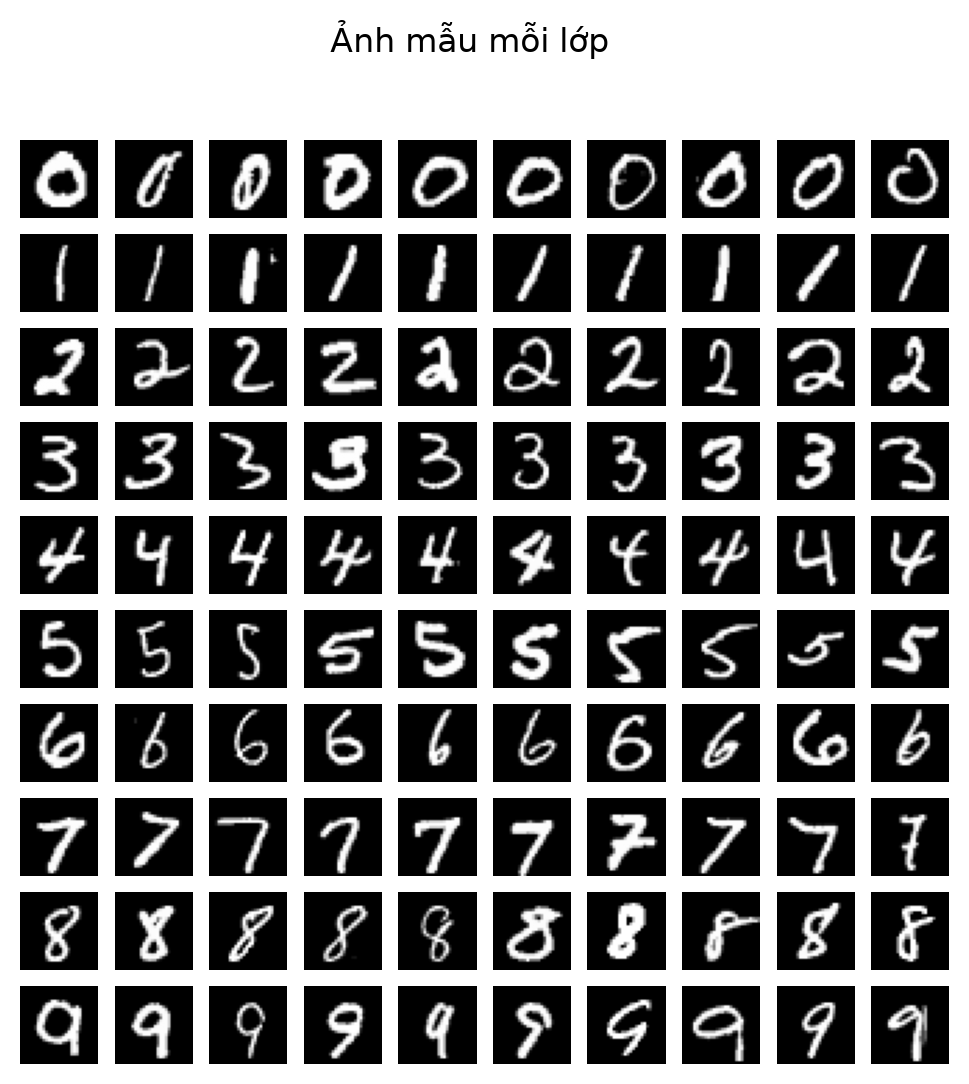
\includegraphics[width=\linewidth]{figures/eda_samples.png}
    \subcaption{Ảnh mẫu (mỗi hàng một lớp)}
  \end{minipage}\hfill
  \begin{minipage}[b]{0.62\linewidth}\centering
    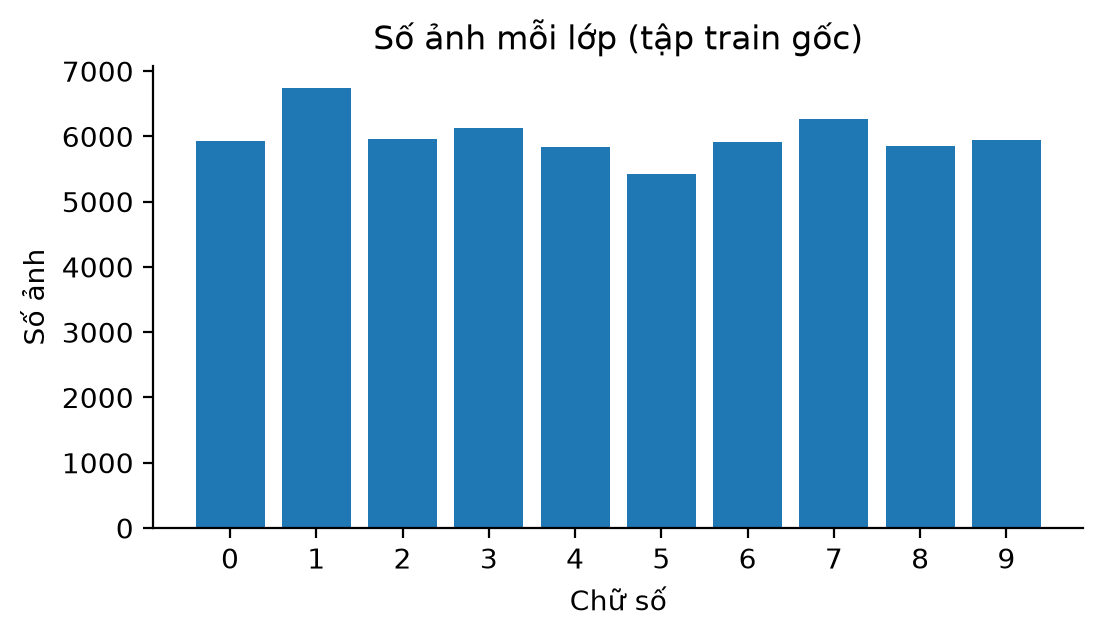
\includegraphics[width=\linewidth]{figures/eda_class_counts.png}
    \subcaption{Số ảnh mỗi lớp trong 60.000 ảnh huấn luyện gốc}
  \end{minipage}
  \caption{(a) Mười ảnh ngẫu nhiên của mỗi chữ số trong tập huấn luyện. (b) Phân bố lớp: ít nhất 5.421 ảnh (số 5), nhiều nhất 6.742 ảnh (số 1).}
  \label{fig:eda1}
\end{figure}

\textbf{Độ đa dạng và phân bố lớp.} Hình~\ref{fig:eda1}a cho thấy nét viết trong cùng lớp khác nhau đáng kể về độ nghiêng, độ dày và kiểu viết (số 4 nét hở hoặc kín, số 7 có hoặc không gạch ngang); các cặp dễ nhầm là 4--9, 3--5--8 và 7--1. Theo Hình~\ref{fig:eda1}b, số mẫu mỗi lớp dao động từ 5.421 (số 5) đến 6.742 (số 1), tỉ lệ lớn nhất/nhỏ nhất là 1,24. Dữ liệu khá cân bằng nên accuracy vẫn có ý nghĩa; nhóm báo cáo thêm precision, recall và F1 macro để mọi lớp có trọng số như nhau.

\begin{figure}[H]
  \centering
  \begin{minipage}{\linewidth}\centering
    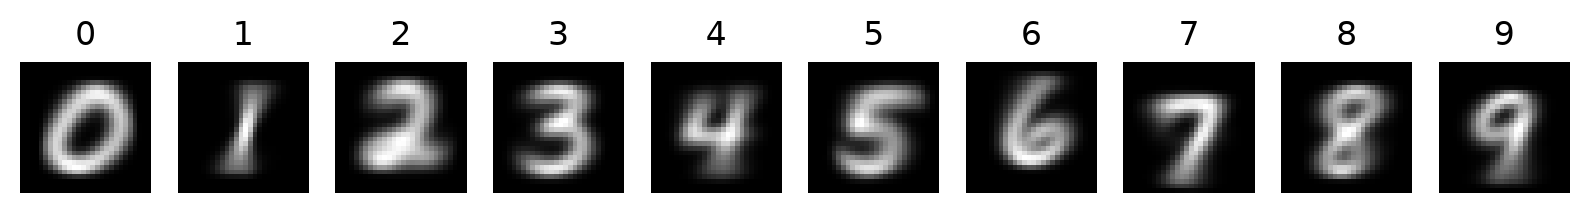
\includegraphics[width=0.92\linewidth]{figures/eda_mean_images.png}
    \subcaption{Ảnh trung bình của từng lớp}
  \end{minipage}\\[4pt]
  \begin{minipage}{\linewidth}\centering
    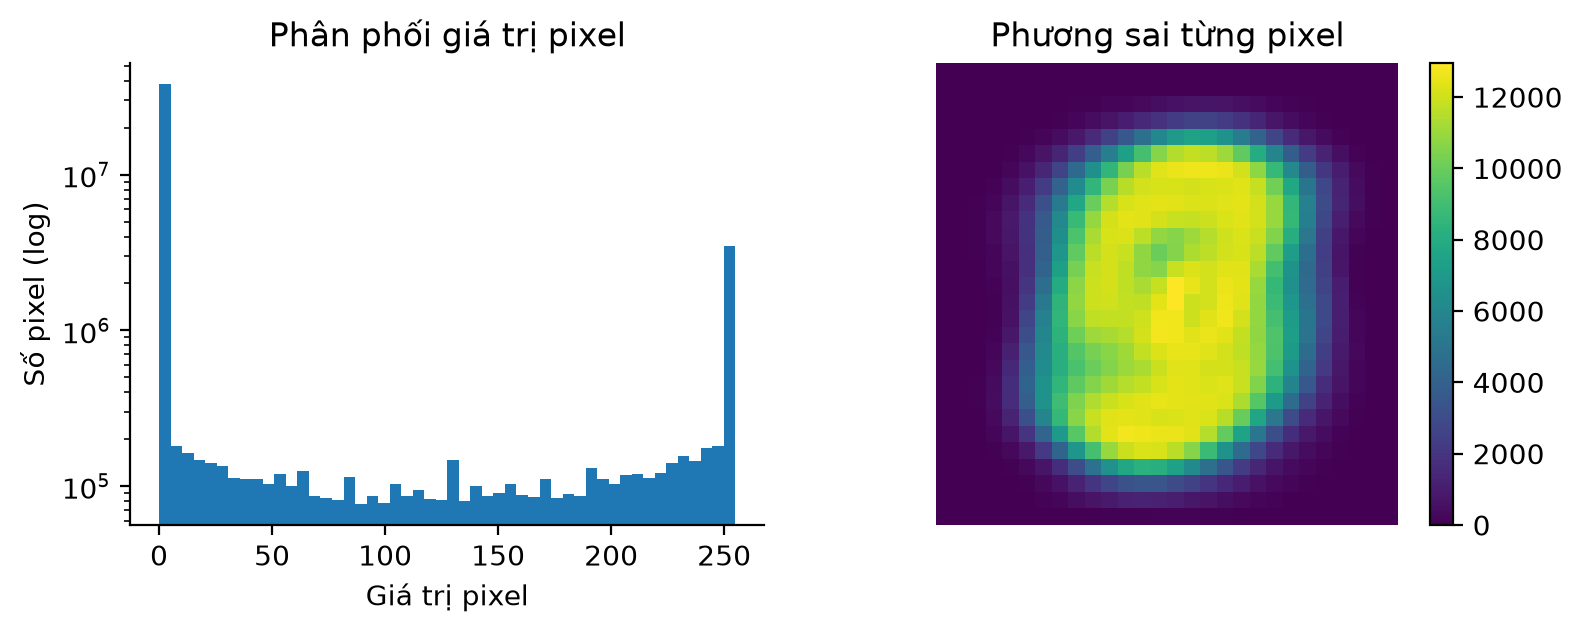
\includegraphics[width=0.8\linewidth]{figures/eda_pixels.png}
    \subcaption{Histogram giá trị pixel (trục tung thang log) và phương sai của từng pixel}
  \end{minipage}
  \caption{Thống kê pixel trên 60.000 ảnh huấn luyện gốc (giá trị 0--255).}
  \label{fig:meanstd}
\end{figure}

\textbf{Giá trị pixel.} Ảnh rất thưa: 80,9\% giá trị pixel bằng 0, và histogram (Hình~\ref{fig:meanstd}b) có hai đỉnh rõ tại 0 (nền) và 255 (lõi nét), các giá trị trung gian chỉ xuất hiện ở viền nét do khử răng cưa. Trung bình mỗi ảnh có khoảng 150 pixel nét; số 1 ít nhất (85,8) và số 0 nhiều nhất (192,0). Bản đồ phương sai cho thấy thông tin tập trung ở vùng giữa ảnh; 67/784 pixel ở viền có phương sai bằng 0, tức luôn bằng 0 trên toàn tập huấn luyện, nên không mang thông tin phân lớp. Ảnh trung bình của từng lớp (Hình~\ref{fig:meanstd}a) đã phân biệt được bằng mắt, gợi ý rằng ngay cả bộ phân lớp tuyến tính cũng có thể đạt kết quả khá; các cặp có ảnh trung bình gần nhau như 4--9 và 3--5--8 được dự báo là dễ nhầm.

\subsection{Tiền xử lý}
\label{sec:prep}
\textbf{Làm phẳng.} Lớp \code{Flattener} biến mỗi ảnh thành vector $\mathbf{x}\in\R^{784}$ theo thứ tự hàng (pixel $(i,j)$ ở vị trí $28i+j$) và ép sang \code{float32} để tránh tràn số khi tính trên \code{uint8}.

\textbf{Chuẩn hoá.} Cả bốn mô hình dùng chung chuẩn hoá min-max $x'=x/255\in[0,1]$. Cách này giữ đặc trưng không âm (điều kiện của Multinomial Na\"{\i}ve Bayes), không cần ước lượng tham số từ dữ liệu nên không có nguy cơ rò rỉ thông tin từ validation/test, và đưa đầu vào về thang đo phù hợp với khởi tạo He của MLP. Với các mô hình softmax, nhãn được mã hoá one-hot.

\subsection{Chia tập}
Tập kiểm thử (10.000 ảnh) được giữ nguyên và chỉ dùng một lần cho đánh giá cuối. Từ 60.000 ảnh huấn luyện, lớp \code{StratifiedSplitter} tách 10\% (6.000 ảnh) làm validation theo cách \emph{phân tầng}: lớp $c$ đóng góp $n_c/10$ mẫu. Vì các giá trị này không nguyên, nhóm dùng phương pháp \emph{phần dư lớn nhất}: làm tròn xuống (tổng 5.996) rồi cộng 1 mẫu cho 4 lớp có phần thập phân lớn nhất (lớp 9, 2, 6, 7), bảo đảm tổng đúng 6.000. Hạt giống cố định (\code{seed = 42}) giúp mọi thành viên dùng chung một cách chia. Validation dùng để chọn siêu tham số và dừng sớm.

\begin{table}[H]
  \centering
  \caption{Ba tập sau tiền xử lý (giá trị pixel đã chia 255).}
  \label{tab:split}
  \small
  \begin{tabular}{lrccc}
    \toprule
    Tập & Số mẫu & Số mẫu mỗi lớp (ít nhất -- nhiều nhất) & Trung bình & Độ lệch chuẩn \\
    \midrule
    Train      & 54.000 & 4.879 (số 5) -- 6.068 (số 1) & 0,131 & 0,308 \\
    Validation & 6.000  & 542 (số 5) -- 674 (số 1)     & 0,131 & 0,308 \\
    Test       & 10.000 & 892 (số 5) -- 1.135 (số 1)   & 0,133 & 0,311 \\
    \bottomrule
  \end{tabular}
\end{table}

Thống kê ba tập rất gần nhau, xác nhận việc chia không làm lệch phân bố. Toàn bộ pipeline được đóng gói trong lớp \code{MNISTPreprocessor}, gọi qua hàm \code{load\_and\_prepare} trong notebook.
% =====================================================================
%  hg.tex — NỘI DUNG BÁO CÁO (chỉ phần thân, KHÔNG có preamble)
%  Dùng trong main.tex:   \input{content/hg}
%  Cần nạp trước trong preamble của main.tex:  \input{content/preamble_hg}
%  Đường dẫn ảnh "figures/..." tính từ thư mục chứa main.tex.
% =====================================================================
% =====================================================================
\section{Phương pháp}
% =====================================================================

Mỗi ảnh $28\times28$ được làm phẳng thành vector $\mathbf{x}\in[0,1]^{D}$ với $D=784$ (giá trị pixel chia 255). Nhãn $y\in\{0,\dots,9\}$, $K=10$ lớp. Phần này trình bày chi tiết hai phương pháp do nhóm phụ trách là Multinomial Naive Bayes và Random Forest; Logistic Regression và MLP được tóm tắt ở mục~\ref{sec:exp}.

% ---------------------------------------------------------------------
\subsection{Multinomial Naive Bayes}
 
\paragraph{Mô hình.} Naive Bayes chọn lớp có xác suất hậu nghiệm lớn nhất theo định lý Bayes, với giả định các pixel độc lập có điều kiện khi biết lớp:
\begin{equation}
\hat y=\argmax_{c}\,P(c\mid\mathbf{x})=\argmax_{c}\,P(c)\prod_{j=1}^{D}P(j\mid c)^{x_j}.
\end{equation}
Mô hình đa thức coi ảnh như một ``túi mực'': cường độ $x_j$ là số lần ``nét mực'' rơi vào pixel $j$, và $\theta_{cj}=P(j\mid c)$ là xác suất một đơn vị mực của lớp $c$ rơi vào pixel $j$, với $\sum_j\theta_{cj}=1$. Cường độ là số thực trong $[0,1]$ chứ không phải số đếm nguyên, nhưng công thức ước lượng vẫn áp dụng được (``số đếm phân số'').
 
\paragraph{Ước lượng tham số.} Gọi $n_c$ là số ảnh của lớp $c$ và $N_{cj}=\sum_{i:y_i=c}x_{ij}$ là tổng mực tại pixel $j$ của lớp đó. Xác suất tiên nghiệm và xác suất pixel có làm trơn Laplace hệ số $\alpha>0$:
\begin{equation}
\pi_c=\frac{n_c}{n},\qquad
\theta_{cj}=\frac{N_{cj}+\alpha}{\sum_{j'}N_{cj'}+\alpha D}.
\end{equation}
Làm trơn tránh $\theta_{cj}=0$ cho các pixel không bao giờ sáng ở một lớp (EDA cho thấy 67/784 pixel luôn bằng 0 trên toàn tập train); nếu không, chỉ một pixel ``lạ'' cũng đưa xác suất của cả lớp về 0.
 
\paragraph{Dự đoán trong miền log.} Tích của 784 xác suất nhỏ gây tràn dưới, nên mọi phép tính được đưa về log:
\begin{equation}
s_c(\mathbf{x})=\log\pi_c+\sum_{j=1}^{D}x_j\log\theta_{cj},\qquad
\hat y=\argmax_c s_c,\qquad
P(c\mid\mathbf{x})=\frac{e^{s_c}}{\sum_{k}e^{s_k}}.
\end{equation}
Xác suất hậu nghiệm được chuẩn hoá bằng softmax ổn định số (trừ $\max_k s_k$ trước khi lấy mũ).
 
\begin{algorithm}[H]
\caption{Multinomial Naive Bayes}\label{alg:nb}
\begin{algorithmic}[1]
\Function{Fit}{$X\in\R^{n\times D}$, $\mathbf{y}$, $\alpha$}
  \For{mỗi lớp $c$}
    \State $X_c\gets$ các hàng của $X$ có nhãn $c$
    \State $\log\pi_c\gets\log(|X_c|/n)$
    \State $\mathbf{N}_c\gets\sum_{\text{hàng}}X_c$ \Comment{vector $D$ chiều}
    \State $\log\boldsymbol\theta_c\gets\log\big((\mathbf{N}_c+\alpha)/(\textstyle\sum\mathbf{N}_c+\alpha D)\big)$
  \EndFor
\EndFunction
\Function{Predict}{$X$}
  \State $S\gets X\,(\log\Theta)^{\top}+\log\boldsymbol\pi$ \Comment{$S\in\R^{n\times K}$, một phép nhân ma trận}
  \State \Return $\argmax$ theo từng hàng của $S$ \quad (hoặc $\mathrm{softmax}(S)$ cho xác suất)
\EndFunction
\end{algorithmic}
\end{algorithm}
 
\paragraph{Chi tiết cài đặt} (\code{naive\_bayes.py}).
Lớp \code{MultinomialNB(alpha)} lưu \code{log\_prior} (kích thước $K$) và \code{log\_feature\_prob} (kích thước $K\times D$). Huấn luyện chỉ cần một vòng lặp qua $K$ lớp với các phép cộng vector, độ phức tạp $O(nD)$. Dự đoán cho cả tập là một phép nhân ma trận \code{X @ log\_feature\_prob.T + log\_prior}, chi phí $O(DK)$ mỗi ảnh. Dữ liệu được ép về \code{float64} trong \code{fit} để tổng $N_{cj}$ trên hàng nghìn ảnh không bị sai số làm tròn của \code{float32}. Nhãn lớp được lưu trong \code{classes} nên \code{predict} trả về nhãn gốc. Mô hình sau huấn luyện chỉ chiếm 0.1\,MB.
 
\paragraph{Cách kiểm chứng.}
\begin{enumerate}
\item \textbf{Đối chiếu tham số với scikit-learn}: huấn luyện lớp \code{MultinomialNB(alpha=1)} của scikit-learn trên cùng dữ liệu \code{float64}, kiểm tra bằng \code{np.allclose} rằng \code{log\_feature\_prob} trùng \code{feature\_log\_prob\_}, \code{log\_prior} trùng \code{class\_log\_prior\_}, \code{predict\_proba} trùng trên tập validation, và tỉ lệ dự đoán trùng nhau là 100\%. Vì công thức xác định (không có ngẫu nhiên), yêu cầu là khớp \emph{tuyệt đối}, không chỉ gần nhau về accuracy.
\item \textbf{Kiểm tra trực quan}: vẽ $\boldsymbol\theta_c$ thành ảnh $28\times28$ (phải giống ``ảnh trung bình'' của chữ số $c$) và bản đồ $\log\boldsymbol\theta_7-\log\boldsymbol\theta_1$ để xem pixel nào ``bỏ phiếu'' cho 7 so với 1. Kết quả ở Hình~\ref{fig:nb_theta}: mỗi $\boldsymbol\theta_c$ là một chữ số mờ đúng hình dạng; trên bản đồ $7-1$, vùng đỏ (ủng hộ 7) nằm ở hai bên và phần đáy ảnh, nơi chữ 1 hầu như không có mực, còn vùng xanh (ủng hộ 1) chạy dọc đường chéo giữa ảnh, trùng với nét của chữ 1.
\end{enumerate}
 
\begin{figure}[H]
\centering
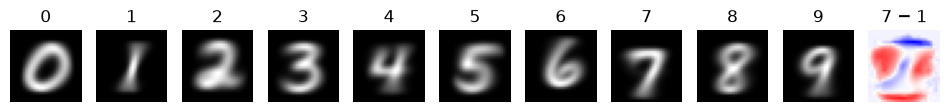
\includegraphics[width=0.95\textwidth]{figures/nb_theta.png}
\caption{Tham số $\boldsymbol\theta_c$ của Multinomial NB vẽ thành ảnh $28\times28$ cho 10 lớp, và hiệu $\log\boldsymbol\theta_7-\log\boldsymbol\theta_1$ (đỏ: ủng hộ 7, xanh: ủng hộ 1).}\label{fig:nb_theta}
\end{figure}


\subsection{Ensemble: Random Forest}
 
\paragraph{Cây quyết định CART với tiêu chí Gini.} Mỗi nút trong hỏi một câu nhị phân ``$x_f\le t$?''; mẫu thoả điều kiện đi sang nhánh trái, còn lại sang phải. Độ vẩn đục Gini của một nút có tỉ lệ lớp $p_k$:
\begin{equation}
G=1-\sum_{k=1}^{K}p_k^2,
\end{equation}
bằng 0 khi nút thuần nhất và đạt tối đa $1-1/K$ khi các lớp chia đều. Với $n$ mẫu tại nút, $n_L$, $n_R$ mẫu ở hai nhánh, phép tách $(f,t)$ được chọn để \emph{độ giảm Gini} lớn nhất:
\begin{equation}
\Delta(f,t)=G_{\text{cha}}-\underbrace{\Big(\tfrac{n_L}{n}G_L+\tfrac{n_R}{n}G_R\Big)}_{\text{Gini có trọng số}}.
\end{equation}
Trọng số $n_L/n$, $n_R/n$ ngăn thuật toán ưa các phép tách ``cắt riêng một mẫu'' (nhánh nhỏ thuần nhưng nhánh lớn vẫn hỗn loạn). Cây phát triển đệ quy tới khi gặp điều kiện dừng; mỗi lá lưu vector tỉ lệ lớp $\mathbf{p}_{\text{lá}}\in\R^K$.
 
\paragraph{Hai nguồn ngẫu nhiên và gộp kết quả.} Random Forest huấn luyện $T$ cây, mỗi cây $b$:
\begin{itemize}
\item học trên một mẫu \textbf{bootstrap} $\mathcal{D}_b$ gồm $n$ mẫu lấy \emph{có hoàn lại}; xác suất một mẫu không được chọn là $(1-1/n)^n\to e^{-1}\approx0.368$;
\item tại \textbf{mỗi nút} chỉ xét $m$ đặc trưng chọn ngẫu nhiên không lặp, với $m=\lfloor\sqrt{D}\rfloor=28$.
\end{itemize}
Hai nguồn này giảm tương quan $\rho$ giữa các cây. Với $T$ cây có phương sai $\sigma^2$, phương sai của trung bình là $\rho\sigma^2+\frac{1-\rho}{T}\sigma^2$: tăng $T$ triệt tiêu số hạng thứ hai, còn giảm $\rho$ làm nhỏ số hạng thứ nhất. Dự đoán dùng \emph{soft voting}:
\begin{equation}
P(c\mid\mathbf{x})=\frac1T\sum_{b=1}^{T}\mathbf{p}^{(b)}_{\text{lá}(\mathbf{x})}[c],\qquad \hat y=\argmax_c P(c\mid\mathbf{x}).
\end{equation}
 
\paragraph{OOB score và độ quan trọng đặc trưng.} Mẫu không nằm trong $\mathcal{D}_b$ là mẫu \emph{out-of-bag} (OOB) của cây $b$. Mỗi mẫu huấn luyện $i$ được dự đoán chỉ bởi các cây $\mathcal{B}_i=\{b: i\notin\mathcal{D}_b\}$, cho ước lượng accuracy trên dữ liệu chưa thấy mà không cần tập riêng:
\begin{equation}
\text{OOB}=\frac{1}{|\{i:\mathcal{B}_i\neq\varnothing\}|}\sum_{i:\mathcal{B}_i\neq\varnothing}\mathbb{1}\Big[\argmax_c\sum_{b\in\mathcal{B}_i}\mathbf{p}^{(b)}(\mathbf{x}_i)[c]=y_i\Big].
\end{equation}
Độ quan trọng của đặc trưng $f$ là tổng $n_{\text{nút}}\cdot\Delta$ qua mọi nút tách theo $f$, chuẩn hoá tổng bằng 1 trong từng cây, rồi lấy trung bình qua các cây.
 
\begin{algorithm}[H]
\caption{Tìm phép tách tốt nhất tại một nút (sắp xếp + tổng cộng dồn)}\label{alg:split}
\begin{algorithmic}[1]
\Function{BestSplit}{$X$, $\mathbf{y}$, tập đặc trưng $F$, $m_{\text{leaf}}$}
  \State $\Delta^*\gets0$;\; $\textit{best}\gets\varnothing$;\; $\mathbf{n}_L\gets(1,\dots,n-1)$;\; $\mathbf{n}_R\gets n-\mathbf{n}_L$
  \For{mỗi $f\in F$}
    \State sắp xếp mẫu theo $x_f$ tăng dần $\to$ $\mathbf{x}^s$, $\mathbf{y}^s$
    \State $H\gets\mathrm{onehot}(\mathbf{y}^s)\in\{0,1\}^{n\times K}$
    \State $C_L\gets\mathrm{cumsum}(H)$ bỏ hàng cuối;\; $C_R\gets\sum H-C_L$ \Comment{số mẫu mỗi lớp hai bên, mọi vị trí}
    \State $\mathbf{g}\gets\big(\mathbf{n}_L\,G(C_L/\mathbf{n}_L)+\mathbf{n}_R\,G(C_R/\mathbf{n}_R)\big)/n$ \Comment{Gini có trọng số, $n-1$ giá trị}
    \State $\textit{valid}_j\gets(x^s_j<x^s_{j+1})\wedge(n_{L,j}\ge m_{\text{leaf}})\wedge(n_{R,j}\ge m_{\text{leaf}})$
    \If{không có $j$ hợp lệ} \textbf{tiếp tục} với $f$ kế tiếp \EndIf
    \State $j^*\gets\argmin_{j\,\text{hợp lệ}}g_j$;\; $\Delta\gets G_{\text{cha}}-g_{j^*}$
    \If{$\Delta>\Delta^*$} $\Delta^*\gets\Delta$;\; $\textit{best}\gets\big(f,\;(x^s_{j^*}+x^s_{j^*+1})/2,\;\Delta\big)$ \EndIf
  \EndFor
  \State \Return \textit{best}
\EndFunction
\end{algorithmic}
\end{algorithm}
 
\begin{algorithm}[H]
\caption{Huấn luyện và dự đoán Random Forest}\label{alg:rf}
\begin{algorithmic}[1]
\Function{Grow}{$X$, $\mathbf{y}$, độ sâu $d$}
  \If{$d\ge d_{\max}$ \textbf{hoặc} $n<m_{\text{split}}$ \textbf{hoặc} $G(\mathbf{y})=0$} \Return Lá$(\text{tỉ lệ lớp của }\mathbf{y})$ \EndIf
  \State $F\gets m$ đặc trưng chọn ngẫu nhiên không lặp
  \State $(f,t,\Delta)\gets$ \Call{BestSplit}{$X,\mathbf{y},F,m_{\text{leaf}}$}
  \If{không tìm được} \Return Lá$(\text{tỉ lệ lớp của }\mathbf{y})$ \EndIf
  \State $\textit{imp}[f]\mathrel{+}=n\cdot\Delta$;\; $M\gets(X_{:,f}\le t)$
  \State \Return Nút$\big(f,t,$ \Call{Grow}{$X_M,\mathbf{y}_M,d{+}1$}, \Call{Grow}{$X_{\neg M},\mathbf{y}_{\neg M},d{+}1$}$\big)$
\EndFunction
\Function{FitForest}{$X$, $\mathbf{y}$, $T$}
  \State mã hoá nhãn về $0..K{-}1$; khởi tạo $\textit{oob\_sum}\in\R^{n\times K}$, $\textit{oob\_cnt}\in\R^n$ bằng 0
  \For{$b=1,\dots,T$}
    \State $\textit{rng}_b\gets$ bộ sinh ngẫu nhiên với hạt giống rút từ \code{random\_state}
    \State $I_b\gets n$ chỉ số ngẫu nhiên có hoàn lại trong $\{0,\dots,n{-}1\}$ \Comment{bootstrap}
    \State $\text{cây}_b\gets$ \Call{Grow}{$X_{I_b},\mathbf{y}_{I_b},0$}
    \State $O\gets\{i\notin I_b\}$;\; $\textit{oob\_sum}[O]\mathrel{+}=\text{cây}_b.\text{proba}(X_O)$;\; $\textit{oob\_cnt}[O]\mathrel{+}=1$
  \EndFor
  \State OOB $\gets$ tỉ lệ $\argmax\textit{oob\_sum}[i]=y_i$ trên các $i$ có $\textit{oob\_cnt}[i]>0$
\EndFunction
\Function{Predict}{$\mathbf{x}$}
  \State \Return $\argmax_c \frac1T\sum_b \text{cây}_b.\text{proba}(\mathbf{x})[c]$ \Comment{mỗi cây: đi từ gốc xuống lá}
\EndFunction
\end{algorithmic}
\end{algorithm}
 
\paragraph{Chi tiết cài đặt} (\code{random\_forest.py}, chỉ dùng NumPy).
\begin{itemize}
\item \textbf{Tìm ngưỡng chính xác, không chia bin.} Cách ngây thơ thử từng ngưỡng và đếm lại tốn $O(n^2)$ mỗi đặc trưng. Thuật toán~\ref{alg:split} sắp xếp một lần ($O(n\log n)$), mã hoá one-hot để biến ``đếm'' thành ``cộng'', rồi dùng \code{np.cumsum} để có số đếm lớp bên trái cho \emph{mọi} vị trí tách trong một lượt; bên phải bằng tổng trừ bên trái. Gini của cả $n-1$ vị trí được tính vector hoá nhờ broadcasting (\code{n\_left[:, None]}).
\item \textbf{Vị trí tách hợp lệ.} Điều kiện \code{xs[:-1] < xs[1:]} loại các vị trí nằm giữa hai giá trị bằng nhau (không ngưỡng nào tách được chúng, rất thường gặp vì nhiều pixel bằng 0); các vị trí không hợp lệ được gán $+\infty$ bằng \code{np.where} trước khi lấy \code{argmin}. Ngưỡng là trung điểm hai giá trị kề nhau. Đặc trưng không có vị trí hợp lệ (pixel hằng) bị bỏ qua; nếu không đặc trưng nào tách được, nút thành lá.
\item \textbf{Mã hoá nhãn và số lớp cố định.} \code{np.unique(y, return\_inverse=True)} đưa nhãn về $0..K{-}1$; $K$ được tính một lần ở rừng và truyền cho mọi cây, nên vector xác suất của mọi lá đều dài $K$ kể cả khi mẫu bootstrap thiếu lớp. \code{classes\_} dùng để đổi ngược về nhãn gốc khi dự đoán.
\item \textbf{Tái lập được.} Mỗi cây có bộ sinh riêng \code{default\_rng(rng.integers(2**31))} rút từ bộ sinh gốc \code{random\_state}; cùng hạt giống cho cùng một rừng.
\item \textbf{Hiệu năng.} Lớp \code{Node} dùng \code{\_\_slots\_\_} để giảm bộ nhớ; duyệt cây khi dự đoán bằng vòng \code{while} (không đệ quy). \code{max\_features} chấp nhận \code{"sqrt"}, \code{"log2"}, số thực (tỉ lệ) hoặc số nguyên và được quy về số nguyên bằng \code{\_resolve\_max\_features}; \code{voting} chọn \code{"soft"} hoặc \code{"hard"}. Dự đoán dùng vòng lặp Python theo từng ảnh nên chậm hơn các mô hình còn lại (khoảng 0.2\,ms/ảnh với 50 cây).
\end{itemize}
 
\paragraph{Cách kiểm chứng.}
\begin{enumerate}
\item \textbf{Tính tay.} Trên ví dụ 10 ảnh một đặc trưng (độ sáng pixel tâm, nhãn $0,0,0,0,1,1,7,1,7,7$), $G_{\text{cha}}=0.66$; in \code{child\_gini} của cả 9 vị trí tách và so với bảng tính tay: ngưỡng $t=0.40$ cho Gini có trọng số $0.300$, $\Delta=0.360$ lớn nhất; các ngưỡng $0.10$, $0.75$, $0.875$ cho $0.525$, $0.417$, $0.475$, khớp hoàn toàn.
\item \textbf{Dữ liệu tổng hợp có đáp án biết trước.} 3 lớp, 2 đặc trưng có ích và 6 đặc trưng nhiễu: rừng cho feature importance $\approx0.30$ và $0.34$ cho hai đặc trưng có ích, $\approx0.06$ cho mỗi đặc trưng nhiễu; accuracy rừng (0.849) vượt một cây (0.782).
\item \textbf{Đối chiếu scikit-learn}: so với lớp \code{RandomForestClassifier} dùng cùng \code{n\_estimators}, \code{max\_depth}, \code{min\_samples\_leaf} và \code{max\_features} $=\sqrt{D}$. Vì có ngẫu nhiên, tiêu chí là accuracy gần nhau chứ không phải trùng từng dự đoán (Bảng~\ref{tab:sklearn}).
\item \textbf{Nhất quán nội tại.} OOB score phải gần accuracy validation, và bản đồ importance phải bằng 0 ở các pixel viền luôn tối. Kết quả: OOB $=0.9549$ so với val $0.9622$ (thấp hơn khoảng 0.7 điểm, đúng kỳ vọng vì mỗi mẫu OOB chỉ được khoảng 37\% số cây bỏ phiếu); 158/784 pixel không bao giờ được dùng để tách (bao gồm 67 pixel luôn bằng 0), và importance tập trung ở vùng tâm nơi các nét chữ phân biệt nhau (Hình~\ref{fig:rf_importance}).
\end{enumerate}
 
\begin{figure}[H]
\centering
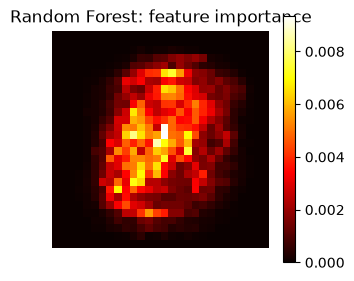
\includegraphics[width=0.4\textwidth]{figures/rf_importance.png}
\caption{Feature importance của Random Forest (50 cây) vẽ thành ảnh $28\times28$.}\label{fig:rf_importance}
\end{figure}

\subsection{Logistic Regression đa lớp (Softmax Regression) bằng Gradient Descent}

\paragraph{Mô tả ý tưởng.}
Logistic Regression phân loại ảnh MNIST thành 10 lớp chữ số từ
$0$ đến $9$. Mỗi lớp có một vector trọng số, có thể hình dung như
một ``tấm khuôn'' dùng để đánh giá mức độ phù hợp của ảnh với chữ số đó.
Mô hình tính điểm số cho từng lớp, chuyển thành xác suất bằng Softmax,
sau đó chọn lớp có xác suất cao nhất. Các trọng số được học bằng
Mini-batch Gradient Descent nhằm giảm hàm mất mát.

\paragraph{Công thức chính và mã giả.}
Với $X\in\mathbb{R}^{n\times784}$,
$W\in\mathbb{R}^{784\times10}$ và $b\in\mathbb{R}^{10}$,
điểm số và xác suất dự đoán được tính bởi:
\[
Z=XW+b,\qquad
P_{ik}=\frac{e^{Z_{ik}}}{\sum_{j=1}^{10}e^{Z_{ij}}}.
\]
Hàm mất mát Cross-Entropy kết hợp điều chuẩn $L_2$:
\[
\mathcal{L}=-\frac{1}{n}\sum_{i=1}^{n}
\log(P_{i,y_i}+\varepsilon)
+\frac{\lambda}{2}\|W\|_F^2.
\]
Với mini-batch gồm $B$ mẫu, gradient và quy tắc cập nhật là:
\[
G=\frac{P-Y}{B},\qquad
\nabla_W=X^\top G+\lambda W,\qquad
\nabla_b=\sum_{i=1}^{B}G_i,
\]
\[
W\leftarrow W-\eta\nabla_W,\qquad
b\leftarrow b-\eta\nabla_b.
\]
Trong đó, $Y$ là nhãn One-hot, $\eta$ là tốc độ học và
$\lambda$ là hệ số điều chuẩn. Nhãn dự đoán:
$\hat y_i=\arg\max_k P_{ik}$.

\begin{algorithm}[H]
\caption{Huấn luyện và dự đoán Logistic Regression}
\label{alg:logistic}
\begin{algorithmic}[1]
\Function{Fit}{$X,y,\lambda,\eta,E,B$}
    \State Khởi tạo $W$ ngẫu nhiên nhỏ, $b\gets 0$
    \For{$e=1,\ldots,E$}
        \State Xáo trộn dữ liệu và chia thành mini-batch
        \For{mỗi mini-batch $(X_I,Y_I)$}
            \State $P\gets\operatorname{Softmax}(X_IW+b)$
            \State $G\gets(P-Y_I)/B$
            \State $\nabla_W\gets X_I^\top G+\lambda W$
            \State $\nabla_b\gets\sum_i G_i$
            \State $W\gets W-\eta\nabla_W$
            \State $b\gets b-\eta\nabla_b$
        \EndFor
        \State Ghi nhận train loss và validation accuracy
    \EndFor
    \State \Return $W,b$
\EndFunction
\Function{Predict}{$X,W,b$}
    \State $P\gets\operatorname{Softmax}(XW+b)$
    \State \Return $\arg\max_k P_{ik}$ với mỗi ảnh $i$
\EndFunction
\end{algorithmic}
\end{algorithm}

\paragraph{Chi tiết cài đặt.}
Mô hình được xây dựng bằng Python và NumPy. Hàm
\texttt{fit()} huấn luyện theo mini-batch; \texttt{predict\_proba()}
trả về xác suất 10 lớp và \texttt{predict()} chọn lớp dự đoán.
Khi tính Softmax, trừ giá trị lớn nhất mỗi hàng trước khi lấy hàm mũ
để hạn chế tràn số. Các siêu tham số gồm \texttt{lr}, \texttt{lam},
\texttt{epochs}, \texttt{batch\_size} và \texttt{seed}.

\paragraph{Cách kiểm chứng.}
\begin{enumerate}
    \item \textbf{Tính toán thủ công.}
    Với ví dụ minh họa ba lớp có $\mathbf z=[1,2,0.5]$,
    Softmax cho $\mathbf P\approx[0.2312,0.6285,0.1403]$.
    Tổng xác suất xấp xỉ $1$, lớp dự đoán là lớp $2$.
    Nếu nhãn đúng là lớp $2$, Cross-Entropy xấp xỉ
    $-\ln(0.6285)=0.4648$. MNIST thực tế sử dụng 10 lớp.

    \item \textbf{Kiểm tra gradient.}
    Trên 20 ảnh, với $\lambda=10^{-3}$, seed $=0$ và
    $\epsilon=10^{-5}$, sai số tương đối lớn nhất trên 10
    trọng số được kiểm tra là $4.90\times10^{-7}<10^{-6}$,
    đạt ngưỡng kiểm tra gradient theo trọng số.

    \item \textbf{Kiểm tra huấn luyện.}
    Sau 20 epoch, train loss giảm từ khoảng $0.408$ xuống
    $0.277$; validation accuracy đạt khoảng $91.65\%$
    tại epoch $19$. Mô hình có xu hướng hội tụ; kết quả
    được minh họa ở Hình~\ref{fig:logistic-training}.

    \item \textbf{Đối chiếu với scikit-learn.}
    So sánh với \texttt{LogisticRegression} của scikit-learn
    trên cùng dữ liệu và cách tiền xử lý; dùng accuracy để
    đánh giá mức độ tương đồng giữa hai mô hình. (Bảng~\ref{tab:sklearn}).
\end{enumerate}

\begin{figure}[H]
    \centering
    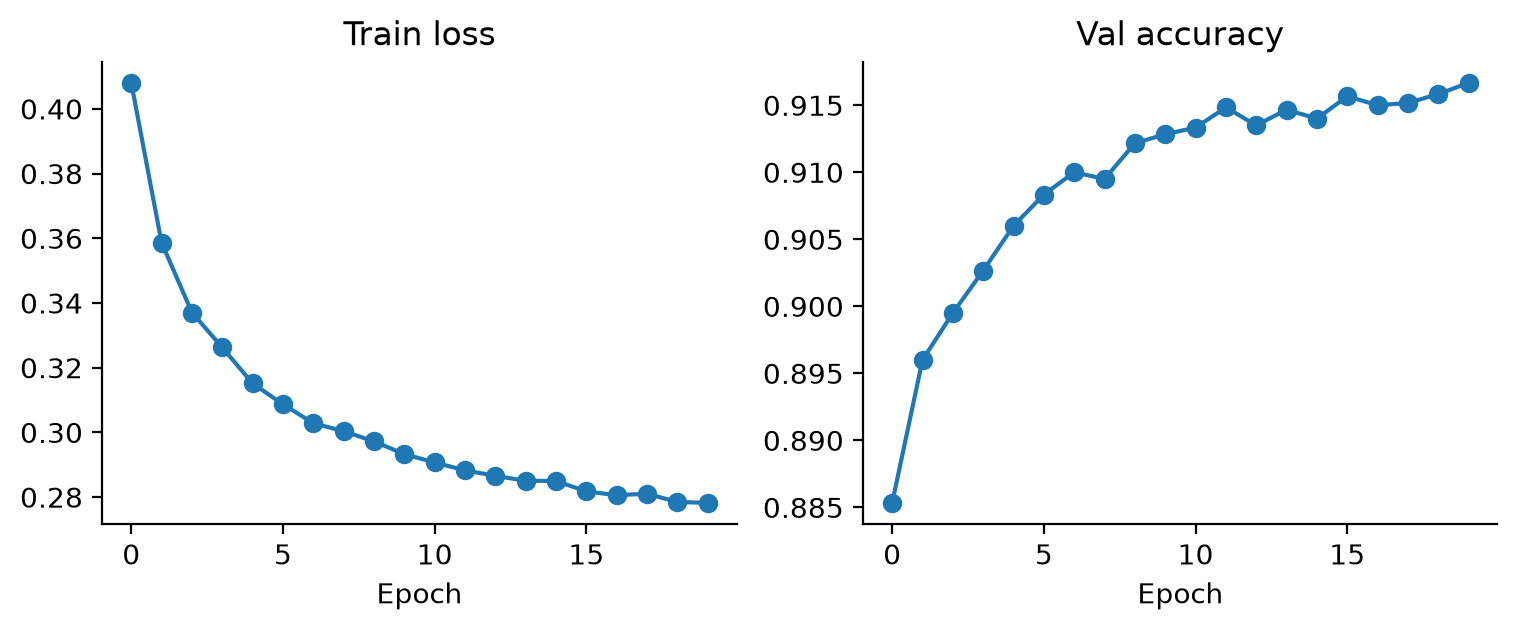
\includegraphics[width=0.72\linewidth]{figures/lr_curve.png}
    \caption{Train loss và validation accuracy của Logistic
    Regression trên MNIST.}
    \label{fig:logistic-training}
\end{figure}

\subsection{Multi-layer Perceptron}
\label{sec:mlp}
% =====================================================================

\paragraph{Kiến trúc và lan truyền xuôi.}
Mạng có $L$ lớp tuyến tính với kích thước $d_0=784, d_1,\dots,d_L=10$ (tham số \code{sizes}). Với một mini-batch $\mathbf{X}\in\R^{n\times 784}$, đặt $\mathbf{A}_0=\mathbf{X}$ và với $l=1,\dots,L$:
\begin{equation}
  \mathbf{Z}_l = \mathbf{A}_{l-1}\mathbf{W}_l + \mathbf{1}\mathbf{b}_l^{\top},\qquad
  \mathbf{A}_l =
  \begin{cases}
    \mathrm{ReLU}(\mathbf{Z}_l)=\max(\mathbf{Z}_l,0), & l<L,\\[2pt]
    \mathrm{softmax}(\mathbf{Z}_l), & l=L,
  \end{cases}
  \label{eq:forward}
\end{equation}
trong đó $\mathbf{W}_l\in\R^{d_{l-1}\times d_l}$, $\mathbf{b}_l\in\R^{d_l}$. Hàm softmax theo từng hàng được tính ổn định số bằng cách trừ giá trị lớn nhất trước khi lấy mũ:
\begin{equation}
  \mathrm{softmax}(\mathbf{z})_k=\frac{e^{z_k-m}}{\sum_{j}e^{z_j-m}},\qquad m=\max_j z_j .
\end{equation}
Phép trừ $m$ không đổi kết quả nhưng tránh tràn số khi $z_k$ lớn. Đầu ra $\mathbf{P}=\mathbf{A}_L$ là ma trận xác suất, nhãn dự đoán là $\hat{y}_i=\arg\max_k P_{ik}$. Kiến trúc cơ sở $(784,128,10)$ có $101.770$ tham số; kiến trúc được chọn $(784,256,128,10)$, có $235.146$ tham số.

\paragraph{Hàm mất mát.}
Với nhãn one-hot $\mathbf{Y}$, hàm mục tiêu là cross-entropy trung bình cộng điều chuẩn L2 (chỉ áp lên trọng số, không áp lên bias):
\begin{equation}
  J(\theta) = -\frac{1}{n}\sum_{i=1}^{n}\sum_{k=1}^{10} Y_{ik}\log P_{ik}
  \;+\; \frac{\lambda}{2}\sum_{l=1}^{L}\lVert\mathbf{W}_l\rVert_F^2 .
  \label{eq:loss}
\end{equation}
Khi cài đặt, $P_{ik}$ được chặn dưới bởi $10^{-12}$ trước khi lấy log để tránh $\log 0$. Trong các thí nghiệm của nhóm, $\lambda=0$ (giá trị mặc định); việc chống khớp quá mức dựa vào dừng sớm.

\paragraph{Lan truyền ngược.}
Với softmax kết hợp cross-entropy, đạo hàm theo đầu vào của lớp ra có dạng gọn $\partial J_{\text{CE}}/\partial\mathbf{Z}_L=(\mathbf{P}-\mathbf{Y})/n$, vì $\partial P_{ik}/\partial Z_{ij} = P_{ik}(\delta_{kj}-P_{ij})$ và $\sum_k Y_{ik}=1$. Đặt $\bm{\Delta}_l=\partial J/\partial\mathbf{Z}_l$, ta có quy tắc truy hồi:
\begin{align}
  \bm{\Delta}_L &= \tfrac{1}{n}(\mathbf{P}-\mathbf{Y}), \label{eq:dL}\\
  \frac{\partial J}{\partial \mathbf{W}_l} &= \mathbf{A}_{l-1}^{\top}\bm{\Delta}_l + \lambda\mathbf{W}_l,\qquad
  \frac{\partial J}{\partial \mathbf{b}_l} = \bm{\Delta}_l^{\top}\mathbf{1}, \label{eq:grad}\\
  \bm{\Delta}_{l-1} &= \big(\bm{\Delta}_l\mathbf{W}_l^{\top}\big)\odot \mathbb{I}[\mathbf{Z}_{l-1}>0], \label{eq:dprev}
\end{align}
với $\odot$ là phép nhân từng phần tử và $\mathbb{I}[\cdot]$ là đạo hàm của ReLU. Hàm \code{backward} cài đặt đúng ba công thức này, dùng lại $\mathbf{A}_l,\mathbf{Z}_l$ đã lưu (cache) trong \code{forward}.

\paragraph{Tối ưu và khởi tạo.}
\textbf{Khởi tạo He} %\cite{he2015}
: $\mathbf{W}_l\sim\mathcal{N}(0,\,2/d_{l-1})$, $\mathbf{b}_l=\mathbf{0}$. Phương sai $2/d_{l-1}$ giữ cho phương sai kích hoạt xấp xỉ không đổi qua các lớp ReLU, tránh tín hiệu bị tắt dần hoặc bùng nổ.

\textbf{SGD với momentum}: với mỗi tham số $\theta$ và gradient $\mathbf{g}$ của mini-batch,
\begin{equation}
  \mathbf{v}\leftarrow \mu\,\mathbf{v}-\eta\,\mathbf{g},\qquad \theta\leftarrow\theta+\mathbf{v},
  \label{eq:momentum}
\end{equation}
với $\eta$ là learning rate, $\mu$ là hệ số momentum và vận tốc $\mathbf{v}$ khởi tạo bằng 0. Momentum tích luỹ hướng của các bước trước, giúp đi nhanh theo hướng ổn định và giảm dao động.

\textbf{Early stopping}: sau mỗi epoch đo accuracy trên validation; nếu không cải thiện sau \code{patience} epoch liên tiếp thì dừng, rồi khôi phục trọng số của epoch tốt nhất. Thuật toán~\ref{alg:mlp} tóm tắt toàn bộ quá trình huấn luyện.

\begin{algorithm}[H]
\caption{Huấn luyện MLP bằng mini-batch SGD + momentum và early stopping (\code{MLP.fit})}
\label{alg:mlp}
\small
\begin{algorithmic}[1]
\Require Dữ liệu $(\mathbf{X},\mathbf{y})$, validation $(\mathbf{X}_v,\mathbf{y}_v)$; siêu tham số $\eta,\mu,\lambda$, số epoch $E$, batch $B$, patience $p$
\Ensure Trọng số $\{\mathbf{W}_l,\mathbf{b}_l\}$ có accuracy validation cao nhất
\State Khởi tạo He cho $\mathbf{W}_l$; $\mathbf{b}_l\gets\mathbf{0}$; $\mathbf{v}^W_l,\mathbf{v}^b_l\gets\mathbf{0}$; $\mathbf{Y}\gets\textsc{OneHot}(\mathbf{y})$
\State $best\gets-1$; $wait\gets 0$
\For{$e=1$ \textbf{to} $E$}
  \State Hoán vị ngẫu nhiên chỉ số mẫu
  \For{mỗi mini-batch $\mathcal{B}$ gồm $B$ chỉ số}
    \State $\mathbf{P}\gets\textsc{Forward}(\mathbf{X}_{\mathcal{B}})$ \Comment{công thức \eqref{eq:forward}, lưu $\mathbf{A}_l,\mathbf{Z}_l$}
    \State $\bm{\Delta}\gets(\mathbf{P}-\mathbf{Y}_{\mathcal{B}})/|\mathcal{B}|$
    \For{$l=L$ \textbf{down to} $1$}
      \State $\mathbf{g}^W_l\gets\mathbf{A}_{l-1}^{\top}\bm{\Delta}+\lambda\mathbf{W}_l$; \quad $\mathbf{g}^b_l\gets\bm{\Delta}^{\top}\mathbf{1}$
      \If{$l>1$} $\bm{\Delta}\gets(\bm{\Delta}\mathbf{W}_l^{\top})\odot\mathbb{I}[\mathbf{Z}_{l-1}>0]$ \EndIf
    \EndFor
    \For{$l=1$ \textbf{to} $L$} \Comment{cập nhật \eqref{eq:momentum}}
      \State $\mathbf{v}^W_l\gets\mu\mathbf{v}^W_l-\eta\mathbf{g}^W_l$; \quad $\mathbf{W}_l\gets\mathbf{W}_l+\mathbf{v}^W_l$ \quad (tương tự với $\mathbf{b}_l$)
    \EndFor
  \EndFor
  \State $acc\gets$ accuracy trên $(\mathbf{X}_v,\mathbf{y}_v)$
  \If{$acc>best$} $best\gets acc$; $wait\gets0$; lưu bản sao trọng số
  \Else\ $wait\gets wait+1$; \textbf{if} $wait\ge p$ \textbf{then break}
  \EndIf
\EndFor
\State Khôi phục trọng số đã lưu
\end{algorithmic}
\end{algorithm}

\paragraph{Chi tiết cài đặt.}
Lớp \code{MLP} (\code{src/mlp.py}) được tự cài hoàn toàn bằng NumPy; PyTorch chỉ dùng để đối chiếu. Một số điểm đáng chú ý:
\begin{itemize}
  \item \textbf{Vector hoá:} mọi phép tính thực hiện trên cả mini-batch bằng phép nhân ma trận, không có vòng lặp theo mẫu.
  \item \textbf{Kiểu số:} mặc định \code{float32} để tăng tốc và giảm bộ nhớ; \code{float64} dùng khi kiểm tra gradient.
  \item \textbf{Dự đoán:} \code{predict\_proba} chạy theo lô 4.096 mẫu và không lưu cache, nên dự đoán trên toàn bộ tập dữ liệu không tốn nhiều RAM.
  \item \textbf{Theo dõi huấn luyện:} \code{history} lưu loss, accuracy (train/validation) và thời gian từng epoch; loss train được cộng dồn từ các lượt forward của mini-batch nên không tốn thêm một lượt duyệt dữ liệu.
  \item \textbf{An toàn số học và lưu/nạp:} tự dừng khi loss là NaN hoặc vô cùng; mô hình cuối được lưu thành file \code{mlp.pkl} (1,9 MB) cho ứng dụng demo.
\end{itemize}

\begin{table}[H]
  \centering
  \caption{Siêu tham số dùng trong notebook. Kiến trúc được chọn trên validation; các siêu tham số còn lại giữ cố định.}
  \label{tab:hparams}
  \small
  \begin{tabular}{llll}
    \toprule
    Siêu tham số & Giá trị & Siêu tham số & Giá trị \\
    \midrule
    Kiến trúc \code{sizes} & khảo sát 4 cấu hình & Kích thước batch $B$ & 128 \\
    Learning rate $\eta$ & 0,05 & Số epoch tối đa $E$ & 15 \\
    Momentum $\mu$ & 0,9 & Patience $p$ & 3 \\
    Hệ số L2 $\lambda$ & 0 & Hạt giống & 42 (khảo sát: 0, 1, 2) \\
    \bottomrule
  \end{tabular}
\end{table}

\paragraph{Kiểm chứng cài đặt.}
\textbf{(1) Ví dụ tính tay.} Với mạng 2--2--2 có trọng số cho trước, đầu vào $(1,2)$ và nhãn lớp 0 (ví dụ trong tài liệu môn học), \code{forward} cho $\mathbf{P}=(0{,}4477;\,0{,}5523)$ và \code{backward} cho $\partial J/\partial\mathbf{W}_1$, $\partial J/\partial\mathbf{W}_2$ trùng với kết quả tính tay đến 4 chữ số thập phân (unit test trong notebook, mục 5.1).

\textbf{(2) Kiểm tra gradient bằng sai phân hữu hạn.} Với mạng nhỏ $(20,16,12,4)$, 8 mẫu ngẫu nhiên, $\lambda=10^{-3}$ và kiểu \code{float64}, gradient từ \code{backward} được so với xấp xỉ sai phân trung tâm tại các phần tử ngẫu nhiên của mọi $\mathbf{W}_l,\mathbf{b}_l$:
\begin{equation}
  g^{\text{num}}=\frac{J(\theta+\epsilon)-J(\theta-\epsilon)}{2\epsilon},\qquad
  \text{err}=\frac{|g^{\text{num}}-g^{\text{bp}}|}{|g^{\text{num}}|+|g^{\text{bp}}|},\qquad \epsilon=10^{-5}.
\end{equation}
Sai số tương đối lớn nhất là $8{,}8\times10^{-8}$, nhỏ hơn ngưỡng thông dụng $10^{-6}$. Kiểm tra được cài trong hàm \code{MLP.gradient\_check} và dùng $\lambda\neq0$ để kiểm cả thành phần L2.

\textbf{(3) Khớp số học với scikit-learn} (\code{tests/kiemchung\_mlp.py}). Sau khi quy đổi $\alpha=\lambda B$ và đặt \code{nesterovs\_momentum=False}, chép trọng số của nhóm sang \code{MLPClassifier}: xác suất dự đoán trùng khớp tuyệt đối, và sau 5 bước SGD trên cùng chuỗi mini-batch, sai lệch trọng số lớn nhất là $1{,}1\times10^{-16}$ (sai số làm tròn của máy).

\textbf{(4) Đối chiếu PyTorch khi huấn luyện đầy đủ} (notebook, mục 5.4). Cùng kiến trúc $(784,128,10)$, khởi tạo Kaiming, SGD momentum 0,9, $\eta=0{,}05$, batch 128, 15 epoch: accuracy validation của bản NumPy là 0,9768, của PyTorch là 0,9775. Chênh lệch 0,07 điểm phần trăm nằm trong mức dao động giữa các hạt giống, do khởi tạo và thứ tự xáo trộn khác nhau.

Ba mức đầu chứng minh từng thành phần (forward, backward, bước cập nhật) đúng về mặt số học; mức cuối cho thấy hành vi khi huấn luyện đầy đủ cũng tương đương với thư viện chuẩn.
% =====================================================================
\section{Thí nghiệm}\label{sec:exp}
% =====================================================================
 
\paragraph{Dữ liệu.} MNIST gồm 60\,000 ảnh train và 10\,000 ảnh test; các lớp gần cân bằng (ít nhất 5\,421 ảnh chữ số 5, nhiều nhất 6\,742 ảnh chữ số 1 trong tập train). Tập train được chia \emph{phân tầng} theo lớp thành 54\,000 ảnh huấn luyện và 6\,000 ảnh validation (hạt giống 42). Pixel được chia 255 (min-max về $[0,1]$), lưu \code{float32}. Mọi siêu tham số được chọn trên validation; tập test chỉ được đánh giá \textbf{một lần} sau khi đã chốt cấu hình (cờ \code{RUN\_TEST}), mỗi mô hình được huấn luyện lại trên 54\,000 ảnh với cấu hình cuối.
 
\paragraph{Môi trường.} Python 3.14.5, NumPy 2.5.4, SciPy 1.18.1, pandas 3.0.6, Matplotlib 3.11.2 trên Windows; CPU/RAM: \todo{điền cấu hình máy}. Cả bốn bộ phân lớp tự cài bằng NumPy; scikit-learn 1.9.1 và PyTorch \todo{phiên bản} chỉ dùng để đối chiếu. Toàn bộ kết quả tái tạo được bằng \emph{Restart \& Run All} trên \code{main.ipynb}.
 
\paragraph{Bốn bộ phân lớp và quy trình chọn siêu tham số.} Bảng~\ref{tab:hparams} tóm tắt không gian tìm kiếm và giá trị được chọn. Với các mô hình có ngẫu nhiên khi huấn luyện (Logistic Regression, MLP), mỗi cấu hình chạy với 3 hạt giống $\{0,1,2\}$ và so sánh trung bình $\pm$ độ lệch chuẩn accuracy validation.
\begin{itemize}
\item \textbf{Multinomial NB}: quét $\alpha$ trên lưới log; không có ngẫu nhiên nên chạy một lần mỗi giá trị.
\item \textbf{Logistic Regression} (softmax, mini-batch GD, cross-entropy $+\frac\lambda2\|W\|^2$): quét learning rate $\eta$, cố định $\lambda=10^{-4}$, 20 epoch, batch 128. Gradient giải tích được kiểm tra bằng sai phân trung tâm (sai số tương đối lớn nhất $4.9\times10^{-7}<10^{-6}$).
\item \textbf{MLP} (ReLU, softmax, SGD momentum 0.9, khởi tạo He, batch 128, tối đa 15 epoch, dừng sớm khi val accuracy không tăng sau 3 epoch và khôi phục trọng số tốt nhất): quét kiến trúc với $\eta=0.05$. Lan truyền ngược được kiểm tra bằng ví dụ tính tay mạng 2--2--2.
\item \textbf{Random Forest}: \code{max\_depth}$=15$, \code{min\_samples\_leaf}$=1$, \code{max\_features}$=\sqrt{D}$, soft voting được cố định trước vì một cây mất khoảng 9\,s huấn luyện trên 54\,000 ảnh; chỉ quét số cây $T$. Đường accuracy theo $T$ lấy từ \emph{một} rừng 50 cây bằng cách cộng dồn xác suất của $k$ cây đầu, không cần huấn luyện lại. OOB score được dùng như ước lượng độc lập thứ hai.
\end{itemize}
 
\begin{table}[H]
\centering\small
\caption{Siêu tham số: không gian tìm kiếm trên validation và giá trị chọn.}\label{tab:hparams}
\begin{tabular}{@{}l l >{\raggedright\arraybackslash}p{5.6cm} l@{}}
\toprule
Mô hình & Siêu tham số quét & Giá trị thử & Chọn \\
\midrule
Multinomial NB & $\alpha$ & $10^{-3},10^{-2},10^{-1},1,10,100$ & $10^{-3}$ \\
Logistic Regression & learning rate $\eta$ ($\times$3 seed) & $10^{-3},10^{-2},10^{-1},1$ & $0.1$ \\
MLP & kiến trúc ($\times$3 seed) & 784-32-10, 784-128-10, 784-512-10, 784-256-128-10 & 784-256-128-10 \\
Random Forest & số cây $T$ & $1,2,5,10,20,30,50$ & 50 \\
\bottomrule
\end{tabular}
\end{table}
 
\paragraph{Thước đo.} Accuracy và macro-F1 (trung bình F1 của 10 lớp) trên train, validation, test; confusion matrix và recall từng lớp trên test; thời gian dự đoán trung bình mỗi ảnh.
% =====================================================================
\section{Kết quả}
% =====================================================================
 
\subsection{Hiệu năng trên ba tập}
 
\begin{table}[H]
\centering\small
\caption{Accuracy và macro-F1 của cấu hình cuối trên train (54\,000), validation (6\,000) và test (10\,000). In đậm: tốt nhất theo cột.}\label{tab:main}
\setlength{\tabcolsep}{4pt}
\begin{tabular}{@{}lcccccccc@{}}
\toprule
& \multicolumn{3}{c}{Accuracy} & \multicolumn{3}{c}{Macro-F1} & Khoảng cách & Dự đoán \\
\cmidrule(lr){2-4}\cmidrule(lr){5-7}
Mô hình & Train & Val & Test & Train & Val & Test & train$-$test & (ms/ảnh) \\
\midrule
Multinomial NB      & 0.8248 & 0.8210 & 0.8364 & 0.8235 & 0.8199 & 0.8349 & $-0.012$ & 0.007 \\
Logistic Regression & 0.9244 & 0.9167 & 0.9213 & 0.9234 & 0.9155 & 0.9201 & $\phantom{-}0.003$ & 0.002 \\
MLP 784-256-128-10  & \textbf{0.9998} & \textbf{0.9813} & \textbf{0.9809} & \textbf{0.9998} & \textbf{0.9813} & \textbf{0.9808} & $\phantom{-}0.019$ & 0.002 \\
Random Forest ($T{=}50$) & 0.9971 & 0.9622 & 0.9645 & 0.9971 & 0.9618 & 0.9642 & $\phantom{-}0.033$ & 0.206 \\
\bottomrule
\end{tabular}
\end{table}
 
Thứ hạng nhất quán trên cả ba tập: MLP $>$ Random Forest $>$ Logistic Regression $>$ Naive Bayes. Accuracy validation và test chênh nhau dưới 1.6 điểm phần trăm với mọi mô hình, cho thấy validation 6\,000 ảnh là thước đo đáng tin để chọn siêu tham số. Hai mô hình tuyến tính/sinh có train $\approx$ test (gần như không overfit, nhưng underfit); MLP và Random Forest gần như thuộc lòng tập train (99.7--99.98\%). Random Forest có OOB score 0.9549, thấp hơn accuracy validation 0.9622 khoảng 0.7 điểm, đúng kỳ vọng vì mỗi mẫu OOB chỉ được khoảng 37\% số cây bỏ phiếu.
 
\subsection{Đối chiếu với thư viện chuẩn}
 
\begin{table}[H]
\centering\small
\caption{Đối chiếu cài đặt tự viết với thư viện chuẩn trên tập validation.}\label{tab:sklearn}
\setlength{\tabcolsep}{4pt}
\begin{tabular}{@{}l l c c >{\raggedright\arraybackslash}p{4.1cm}@{}}
\toprule
Mô hình & Đối chiếu với & Tự cài & Thư viện & Tiêu chí / nhận xét \\
\midrule
Multinomial NB & sklearn \code{MultinomialNB} & 0.8210 & 0.8210 & $\log\theta$, $\log\pi$, xác suất khớp (\code{allclose}); dự đoán trùng 100\% \\
Logistic Regression & sklearn \code{LogisticRegression} & 0.9167 & 0.9183 & quy đổi $C=1/(n\lambda)$; chênh 0.16 điểm \\
MLP 784-128-10 & PyTorch (SGD momentum) & 0.9768 & 0.9775 & cùng kiến trúc, khởi tạo He; chênh 0.07 điểm \\
Random Forest ($T{=}50$) & sklearn \code{RandomForestClassifier} & 0.9622 & 0.9608 & cùng tham số; chênh 0.14 điểm \\
\bottomrule
\end{tabular}
\end{table}
 
Naive Bayes khớp tuyệt đối với scikit-learn (khi so trên \code{float64}). Ba mô hình còn lại có thành phần ngẫu nhiên hoặc bộ tối ưu khác nhau nên chỉ cần chênh lệch nhỏ; mọi chênh lệch đều dưới 0.2 điểm phần trăm, và Random Forest tự cài thậm chí nhỉnh hơn bản scikit-learn ở hạt giống này. Kết quả này xác nhận hai cài đặt của nhóm đúng về mặt thuật toán.
 
\subsection{Ảnh hưởng của siêu tham số}
 
\begin{figure}[H]
\centering
\begin{subfigure}[b]{0.36\textwidth}\centering
  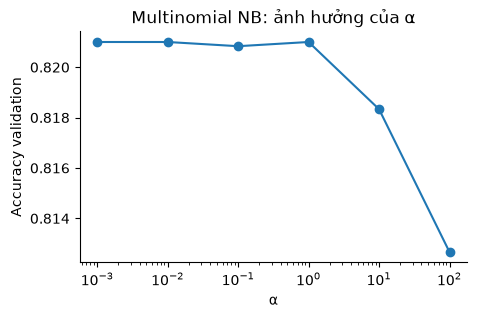
\includegraphics[width=\linewidth]{figures/nb_alpha.png}
  \caption{Multinomial NB: hệ số làm trơn $\alpha$.}\label{fig:nb_alpha}
\end{subfigure}\hspace{1.5cm}
\begin{subfigure}[b]{0.36\textwidth}\centering
  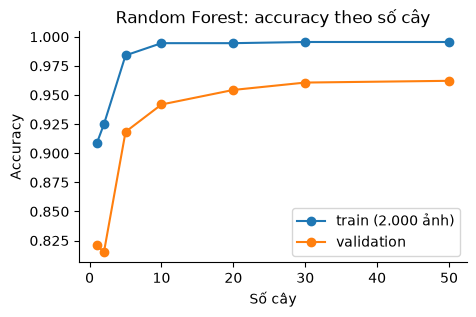
\includegraphics[width=\linewidth]{figures/rf_trees.png}
  \caption{Random Forest: accuracy theo số cây.}\label{fig:rf_trees}
\end{subfigure}\\[4pt]
\begin{subfigure}[b]{0.56\textwidth}\centering
  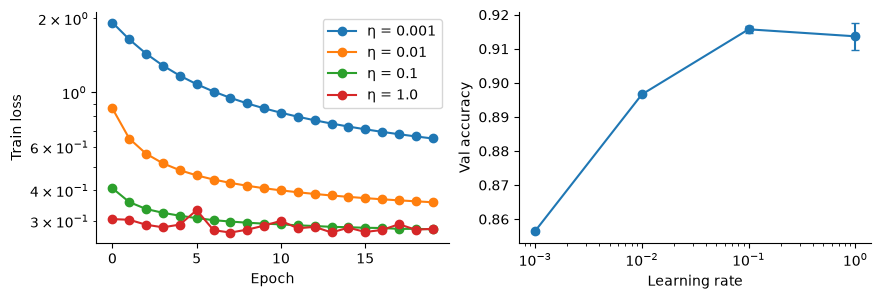
\includegraphics[width=\linewidth]{figures/lr_sweep.png}
  \caption{Logistic Regression: loss theo epoch và val accuracy theo $\eta$ (3 seed).}\label{fig:lr_sweep}
\end{subfigure}\hfill
\begin{subfigure}[b]{0.33\textwidth}\centering
  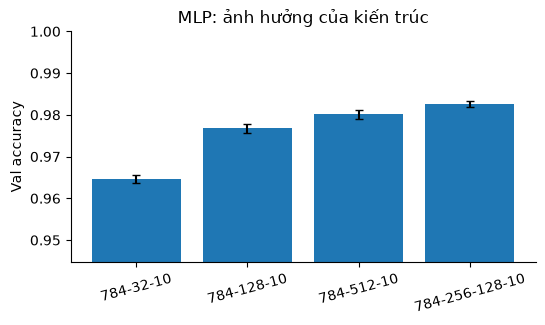
\includegraphics[width=\linewidth]{figures/mlp_arch.png}
  \caption{MLP: kiến trúc (3 seed).}\label{fig:mlp_arch}
\end{subfigure}
\caption{Accuracy validation theo siêu tham số của bốn bộ phân lớp. Thanh lỗi: độ lệch chuẩn qua 3 hạt giống.}\label{fig:hparams}
\end{figure}
 
\begin{itemize}
\item \textbf{NB (Hình~\ref{fig:nb_alpha})}: accuracy gần như phẳng ($\approx0.821$) với $\alpha\le1$, rồi giảm còn 0.818 ở $\alpha=10$ và 0.813 ở $\alpha=100$. Tổng mực mỗi lớp lên tới hàng trăm nghìn, nên $\alpha$ nhỏ hầu như không đổi $\theta$; $\alpha$ lớn kéo mọi $\theta_{cj}$ về phân phối đều, xoá đi hình dạng chữ số. Giá trị $10^{-3}$ được chọn nhưng khác biệt với $\alpha=1$ là không đáng kể.
\item \textbf{Logistic Regression (Hình~\ref{fig:lr_sweep})}: $\eta=10^{-3}$ hội tụ quá chậm (0.856 sau 20 epoch), $\eta=10^{-2}$ đạt 0.897; $\eta=0.1$ đạt cao nhất (0.916) với độ lệch nhỏ. $\eta=1$ có trung bình tương đương nhưng loss dao động mạnh theo epoch và độ lệch chuẩn giữa các seed lớn hơn, nên $\eta=0.1$ được chọn.
\item \textbf{MLP (Hình~\ref{fig:mlp_arch})}: accuracy tăng theo dung lượng mô hình: 0.965 (32 nơ-ron) $\to$ 0.977 (128) $\to$ 0.980 (512) $\to$ 0.983 (256-128). Mạng hai lớp ẩn tốt nhất dù có ít tham số hơn mạng 784-512-10 (235\,146 so với 407\,050).
\item \textbf{Random Forest (Hình~\ref{fig:rf_trees})}: một cây đạt khoảng 0.82, hai cây còn thấp hơn (soft voting của 2 cây dễ hoà), 10 cây đạt 0.94, rồi bão hoà quanh 0.96 từ 30 cây. Accuracy train (đo trên 2\,000 ảnh train) đạt $\approx$1.0 từ 10 cây: khoảng cách train--validation không thu hẹp khi thêm cây, vì thêm cây chỉ giảm phương sai chứ không giảm độ phức tạp từng cây.
\end{itemize}
 
\subsection{Confusion matrix trên tập test}
 
\begin{figure}[H]
\centering
\begin{subfigure}[b]{0.245\textwidth}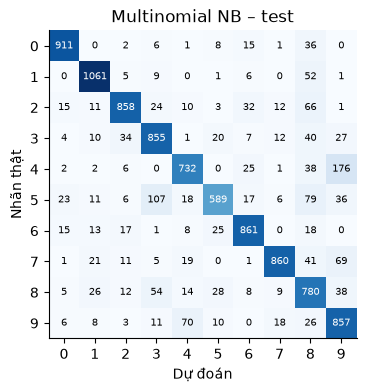
\includegraphics[width=\linewidth]{figures/cm_test_nb.png}\end{subfigure}\hfill
\begin{subfigure}[b]{0.245\textwidth}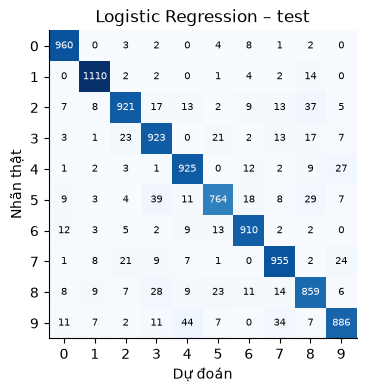
\includegraphics[width=\linewidth]{figures/cm_test_lr.png}\end{subfigure}\hfill
\begin{subfigure}[b]{0.245\textwidth}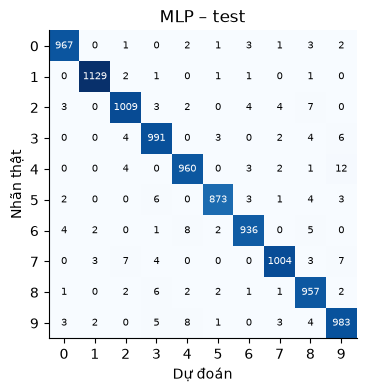
\includegraphics[width=\linewidth]{figures/cm_test_mlp.png}\end{subfigure}\hfill
\begin{subfigure}[b]{0.245\textwidth}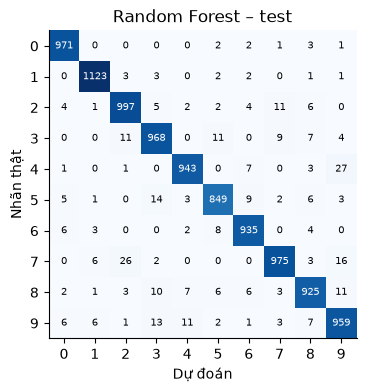
\includegraphics[width=\linewidth]{figures/cm_test_rf.png}\end{subfigure}
\caption{Confusion matrix trên 10\,000 ảnh test (hàng: nhãn thật, cột: dự đoán). Tổng số lỗi: NB 1\,636, LR 787, MLP 191, RF 355.}\label{fig:cm}
\end{figure}
 
\begin{table}[H]
\centering\small
\caption{Recall từng lớp trên tập test, tính từ Hình~\ref{fig:cm}. In đậm: lớp khó nhất của mỗi mô hình.}\label{tab:recall}
\begin{tabular}{@{}lcccccccccc@{}}
\toprule
Mô hình & 0 & 1 & 2 & 3 & 4 & 5 & 6 & 7 & 8 & 9 \\
\midrule
Multinomial NB      & 0.930 & 0.935 & 0.831 & 0.847 & 0.745 & \textbf{0.660} & 0.899 & 0.837 & 0.801 & 0.849 \\
Logistic Regression & 0.980 & 0.978 & 0.892 & 0.914 & 0.942 & \textbf{0.857} & 0.950 & 0.929 & 0.882 & 0.878 \\
MLP                 & 0.987 & 0.995 & 0.978 & 0.981 & 0.978 & 0.979 & 0.977 & 0.977 & 0.983 & \textbf{0.974} \\
Random Forest       & 0.991 & 0.989 & 0.966 & 0.958 & 0.960 & 0.952 & 0.976 & \textbf{0.948} & 0.950 & 0.950 \\
\bottomrule
\end{tabular}
\end{table}
 
\begin{table}[H]
\centering\small
\caption{Số lỗi của các cặp hay nhầm (cộng cả hai chiều, ví dụ $4\leftrightarrow9$ = $4\to9$ + $9\to4$) trên tập test.}\label{tab:pairs}
\begin{tabular}{@{}lcccccc@{}}
\toprule
Mô hình & $4\leftrightarrow9$ & $3\leftrightarrow5$ & $7\leftrightarrow9$ & $2\leftrightarrow7$ & $2\to8$ & Tổng lỗi \\
\midrule
Multinomial NB      & 246 (176+70) & 127 (20+107) & 87 & 23 & 66 & 1\,636 \\
Logistic Regression & 71 (27+44)   & 60 (21+39)   & 58 & 34 & 37 & 787 \\
MLP                 & 20 (12+8)    & 9 (3+6)      & 10 & 11 & 7  & 191 \\
Random Forest       & 38 (27+11)   & 25 (11+14)   & 19 & 37 (11+26) & 6 & 355 \\
\bottomrule
\end{tabular}
\end{table}
 
Ở cả bốn mô hình, phần lớn khối lượng nằm trên đường chéo; chữ số 0 và 1 dễ nhất (recall $\ge0.93$ ở mọi mô hình). Cặp $4\leftrightarrow9$ là nguồn lỗi chung lớn nhất. Naive Bayes có các cột ``hút'' lỗi rõ rệt: cột 8 nhận 396 ảnh sai và cột 9 nhận 348 ảnh sai; riêng chữ số 5 bị đoán thành 3 tới 107 lần, khiến recall lớp 5 chỉ 0.66.
% =====================================================================
\section{Thảo luận}
% =====================================================================
 
\subsection{So sánh bốn phương pháp}
 
\paragraph{Độ chính xác và thiên kiến mô hình.} Thứ tự accuracy phản ánh mức độ linh hoạt của biên quyết định. Naive Bayes và Logistic Regression đều có biên \emph{tuyến tính} trong không gian pixel (điểm số NB $s_c=\log\pi_c+\mathbf{x}^\top\log\boldsymbol\theta_c$ cũng tuyến tính theo $\mathbf{x}$), nhưng NB ước lượng tham số theo giả định độc lập pixel và không tối ưu trực tiếp cho phân lớp, còn LR tối ưu cross-entropy một cách phân biệt. Cùng một họ biên tuyến tính, LR giảm lỗi test từ 1\,636 xuống 787, tức hơn một nửa. Cả hai có khoảng cách train--test gần 0: đây là \emph{underfit}, mô hình quá đơn giản chứ không phải học thuộc. MLP và Random Forest có biên phi tuyến, đạt 96--98\% nhưng đổi lại khoảng cách train--test lớn hơn (1.9 và 3.3 điểm).
 
\paragraph{MLP so với Random Forest.} Hai mô hình phi tuyến đều gần như thuộc lòng tập train, nhưng MLP tổng quát hoá tốt hơn: lỗi test 191 so với 355. Mỗi nút của cây chỉ hỏi \emph{một} pixel so với một ngưỡng, nên biên quyết định gồm các mặt cắt song song trục; một nét bút dịch đi 1--2 pixel làm thay đổi hàng loạt câu trả lời. Các nơ-ron ẩn của MLP là tổ hợp tuyến tính của mọi pixel, học được các ``mẫu nét'' bền hơn với biến dạng nhỏ. Recall của MLP cũng đồng đều nhất giữa các lớp (0.974--0.995), trong khi Random Forest có các lớp 7, 8, 9 thấp hơn hẳn lớp 0, 1.
 
\paragraph{Chi phí và khả năng diễn giải.}
\begin{table}[H]
\centering\small
\caption{So sánh thực tiễn bốn bộ phân lớp (cấu hình cuối).}\label{tab:practical}
\begin{tabular}{@{}lcccl@{}}
\toprule
Mô hình & Test acc. & Dự đoán (ms/ảnh) & Kích thước file & Diễn giải \\
\midrule
Multinomial NB      & 0.836 & 0.007 & 0.1\,MB  & bản đồ $\theta_c$, hiệu $\log\theta_7-\log\theta_1$ \\
Logistic Regression & 0.921 & 0.002 & 0.1\,MB  & trọng số mỗi lớp vẽ thành ảnh \\
MLP                 & 0.981 & 0.002 & 1.9\,MB  & khó, chỉ gián tiếp \\
Random Forest       & 0.965 & 0.206 & 35.1\,MB & feature importance từng pixel \\
\bottomrule
\end{tabular}
\end{table}
Naive Bayes huấn luyện tức thì (một lượt cộng dồn) và không có siêu tham số nhạy cảm, phù hợp làm đường cơ sở. Random Forest không cần chuẩn hoá dữ liệu, không cần learning rate, có OOB score miễn phí, nhưng là mô hình nặng nhất: file 35\,MB (lưu hàng chục nghìn nút) và dự đoán chậm hơn MLP khoảng 100 lần do duyệt cây bằng vòng lặp Python. MLP cho accuracy cao nhất với chi phí dự đoán ngang mô hình tuyến tính, đổi lại cần chọn learning rate, kiến trúc và dừng sớm, và khó diễn giải nhất.
 
\subsection{Phân tích lỗi}
 
\paragraph{Các cặp nhầm có nguyên nhân hình học.} Bảng~\ref{tab:pairs} cho thấy các cặp hay nhầm giống nhau giữa các mô hình, chỉ khác về độ lớn. $4\leftrightarrow9$ là cặp khó nhất ở mọi mô hình: chữ 4 viết ``đóng'' phần trên gần như trùng chữ 9, chỉ khác nét nối nhỏ ở đỉnh. $3\leftrightarrow5$ và $7\leftrightarrow9$ chia sẻ phần lớn nét (đường cong dưới của 3 và 5; nét chéo của 7 và thân 9). Điều này khớp với EDA: ảnh trung bình của các cặp này giống nhau nhất.
 
\paragraph{Vì sao Naive Bayes lỗi theo kiểu ``hút về một lớp''.} Điểm NB là tổng mực có trọng số $\log\theta_{cj}$, nên lớp có ``bản đồ mực'' rộng và phủ nhiều vùng (8 phủ gần hết vùng tâm, 9 phủ phần trên và thân) nhận điểm cao cho rất nhiều ảnh lạ, giải thích cột 8 và cột 9 nhận nhiều lỗi. Chữ 5 bị đoán thành 3 (107 lần) vì phần dưới hai chữ gần trùng, còn phần trên khác biệt chỉ chiếm ít pixel. Giả định độc lập pixel không cho NB nhận ra rằng một nét nối liền (đặc trưng của 4 mở so với 9 đóng) quan trọng hơn tổng lượng mực.
 
\paragraph{Random Forest và lỗi $7\to2$.} Random Forest có lỗi $7\to2$ (26 ảnh) nhiều hơn cả Logistic Regression (21). Chữ 7 có gạch ngang giữa hoặc nét dưới cong sang phải có phân bố pixel giống chữ 2 ở phần dưới ảnh; vì mỗi nút chỉ xét một pixel, các cây dễ ``rẽ'' theo vài pixel ở đáy ảnh. Đây là biểu hiện của tính nhạy với vị trí nét đã nêu ở trên.
 
\begin{figure}[H]
\centering
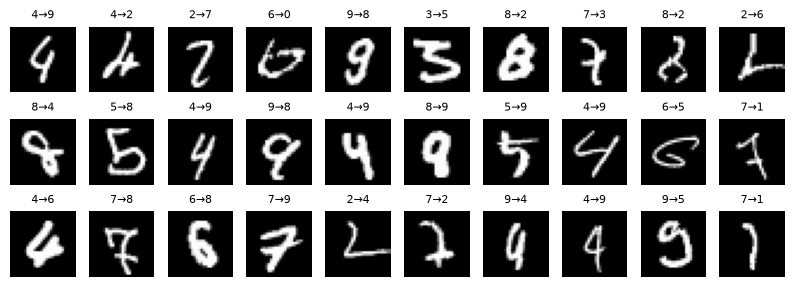
\includegraphics[width=0.9\textwidth]{figures/errors_test.png}
\caption{30 ảnh test đầu tiên bị MLP (mô hình tốt nhất) đoán sai, ghi ``nhãn thật $\to$ dự đoán''.}\label{fig:errors}
\end{figure}
 
\paragraph{Lỗi còn lại của MLP phần lớn là ảnh thật sự mơ hồ.} Trong Hình~\ref{fig:errors}, nhiều ảnh khó với cả người đọc: các chữ 4 có đỉnh khép kín bị đọc là 9 (xuất hiện 5 lần trong 30 ảnh), chữ 2 viết như chữ L (bị đọc thành 6 hoặc 4), chữ 6 viết nghiêng như số 0 hoặc 5, chữ 7 có gạch ngang đọc thành 2 hoặc 3. Một số ảnh có thể bị gán nhãn sai từ gốc. Với 191 lỗi trên 10\,000 ảnh, phần cải thiện còn lại khó đạt được bằng mô hình chỉ nhìn pixel độc lập vị trí như MLP.
 
\subsection{Hạn chế}
 
\begin{itemize}
\item \textbf{Tìm kiếm siêu tham số hạn chế.} Mỗi mô hình chỉ quét một siêu tham số chính. Random Forest cố định \code{max\_depth}$=15$, \code{min\_samples\_leaf}$=1$ và \code{max\_features}$=\sqrt D$ vì chi phí huấn luyện; chưa thử \code{"log2"}, cây sâu hơn hay lá lớn hơn, nên khoảng cách train--test 3.3 điểm có thể còn thu hẹp được. MLP chưa quét learning rate và $\lambda$ (cấu hình cuối dùng $\lambda=0$). Đường theo số cây chỉ lấy từ một rừng, một hạt giống.
\item \textbf{Một lần chia dữ liệu, một hạt giống cho cấu hình cuối.} Accuracy test báo cáo từ một lần huấn luyện; không có khoảng tin cậy. Với 10\,000 ảnh test, sai số chuẩn của accuracy khoảng $\sqrt{p(1-p)/10^4}\approx0.13$--0.37 điểm phần trăm, nên chênh lệch giữa các mô hình trong báo cáo đều có ý nghĩa, nhưng chênh lệch nhỏ khi đối chiếu với thư viện (Bảng~\ref{tab:sklearn}) nằm trong biên độ ngẫu nhiên. Mô hình cuối chỉ huấn luyện trên 54\,000 ảnh, chưa gộp lại validation.
\item \textbf{Hiệu năng cài đặt Random Forest.} Dự đoán bằng vòng lặp Python từng ảnh làm Random Forest chậm nhất (0.2\,ms/ảnh) và huấn luyện tuần tự từng cây (khoảng 9\,s/cây, $\approx$7.5 phút cho 50 cây). Có thể vector hoá việc duyệt cây bằng cách lưu cây dạng mảng và xử lý theo lô, hoặc huấn luyện song song các cây vì chúng độc lập.
\item \textbf{Biểu diễn đầu vào thô.} Cả bốn mô hình nhìn ảnh như vector 784 pixel độc lập vị trí. Thí nghiệm độ bền trong notebook cho thấy khi dịch ảnh 3 pixel theo đường chéo, accuracy test giảm còn 0.11--0.20 với cả bốn mô hình không dùng tăng cường dữ liệu; tăng cường dữ liệu nâng MLP lên 0.78 nhưng Random Forest chỉ lên 0.37. Mạng tích chập (CNN) với tính bất biến tịnh tiến sẵn có mới giải quyết triệt để vấn đề này.
\item \textbf{Lệch miền.} Trên tập 2\,980 chữ số do 30 người Việt viết (đánh giá trên phần người viết giữ lại, trung bình 3 lần chia), accuracy khi chỉ huấn luyện bằng MNIST giảm mạnh: MLP 0.894, Random Forest 0.688, Logistic Regression 0.690, NB 0.575. Kết quả trên MNIST vì vậy đánh giá quá cao khả năng dùng thực tế; Random Forest giảm nhiều nhất (từ 0.962 xuống 0.688), nhất quán với nhận xét về độ nhạy theo vị trí pixel.
\item \textbf{Giả định của Naive Bayes.} Coi cường độ pixel thực là ``số đếm'' và giả định pixel độc lập đều không đúng với ảnh chữ viết, nơi các pixel lân cận tương quan mạnh. Đây là giới hạn của mô hình, không phải của cài đặt (đã khớp tuyệt đối với scikit-learn).
\end{itemize}
\section{Thí nghiệm mở rộng}
Đánh giá khả năng nhận dạng chữ số viết tay của mô hình trên dữ liệu người Việt được nhóm thu thập qua ba thí nghiệm: (a) huấn luyện bằng MNIST; (b) bổ sung data augmentation; (c) kết hợp MNIST với một phần dữ liệu người Việt. Qua đó, đánh giá ảnh hưởng của lệch miền dữ liệu, hiệu quả cải thiện và xây dựng demo vẽ chữ số trực tiếp.
\subsection{Tập chữ số Việt}
\subsubsection{Thu thập và xử lý dữ liệu}
Mỗi người viết điền một phiếu in A4 gồm lưới $10\times10$ ô: mỗi hàng là một chữ số từ 0 đến 9, viết 10 lần theo cách tự nhiên, rồi ký xác nhận đồng ý cho sử dụng dữ liệu. Phiếu có bốn ô đen ở bốn góc làm dấu định vị. Nhóm thu được 30 phiếu từ 30 người viết (mã W01--W30), chụp bằng điện thoại.

Module \code{src/vn\_digits.py} chuyển ảnh phiếu sang định dạng MNIST qua các bước ở Hình~\ref{fig:vnpipe}. Bước cuối lặp lại đúng quy trình tạo MNIST (khung $20\times20$, căn khối tâm vào ảnh $28\times28$), nên khác biệt còn lại chủ yếu là khác biệt về nét viết chứ không phải do định dạng. Cả 3.000 ô đều có chữ (không ô trống); sau khi xem lại từng phiếu, nhóm loại 20 ô viết nhầm, gạch xoá hoặc bẩn (ghi trong \code{data/vn\_exclude.csv}), còn lại \textbf{2.980 ảnh}, mỗi lớp từ 294 đến 300 ảnh.

\begin{figure}[H]
\centering
\begin{tikzpicture}[
  box/.style={draw,rounded corners=2pt,fill=blue!6,align=center,font=\footnotesize,minimum height=1.05cm,text width=2.05cm},
  arr/.style={-{Stealth[length=2mm]},thick}, node distance=0.35cm]
  \node[box] (a) {Ảnh chụp\\phiếu};
  \node[box,right=of a] (b) {Tìm 4 ô đen,\\nắn phẳng\\phối cảnh};
  \node[box,right=of b] (c) {Cắt 100 ô\\theo lưới,\\bỏ lề ô};
  \node[box,right=of c] (d) {Tách nét khỏi\\nền, đảo màu\\(nền đen)};
  \node[box,right=of d] (e) {Cắt khung\\bao, thu về\\$20\times20$};
  \node[box,right=of e] (f) {Căn khối tâm\\vào $28\times28$};
  \foreach \u/\v in {a/b,b/c,c/d,d/e,e/f} \draw[arr] (\u) -- (\v);
\end{tikzpicture}
\caption{Quy trình chuyển ảnh chụp phiếu thành ảnh chữ số theo định dạng MNIST (\code{review\_sheet}, \code{process\_sheet}, \code{build\_dataset}).}
\label{fig:vnpipe}
\end{figure}

\begin{figure}[H]
  \centering
  \begin{minipage}[c]{0.27\linewidth}\centering
    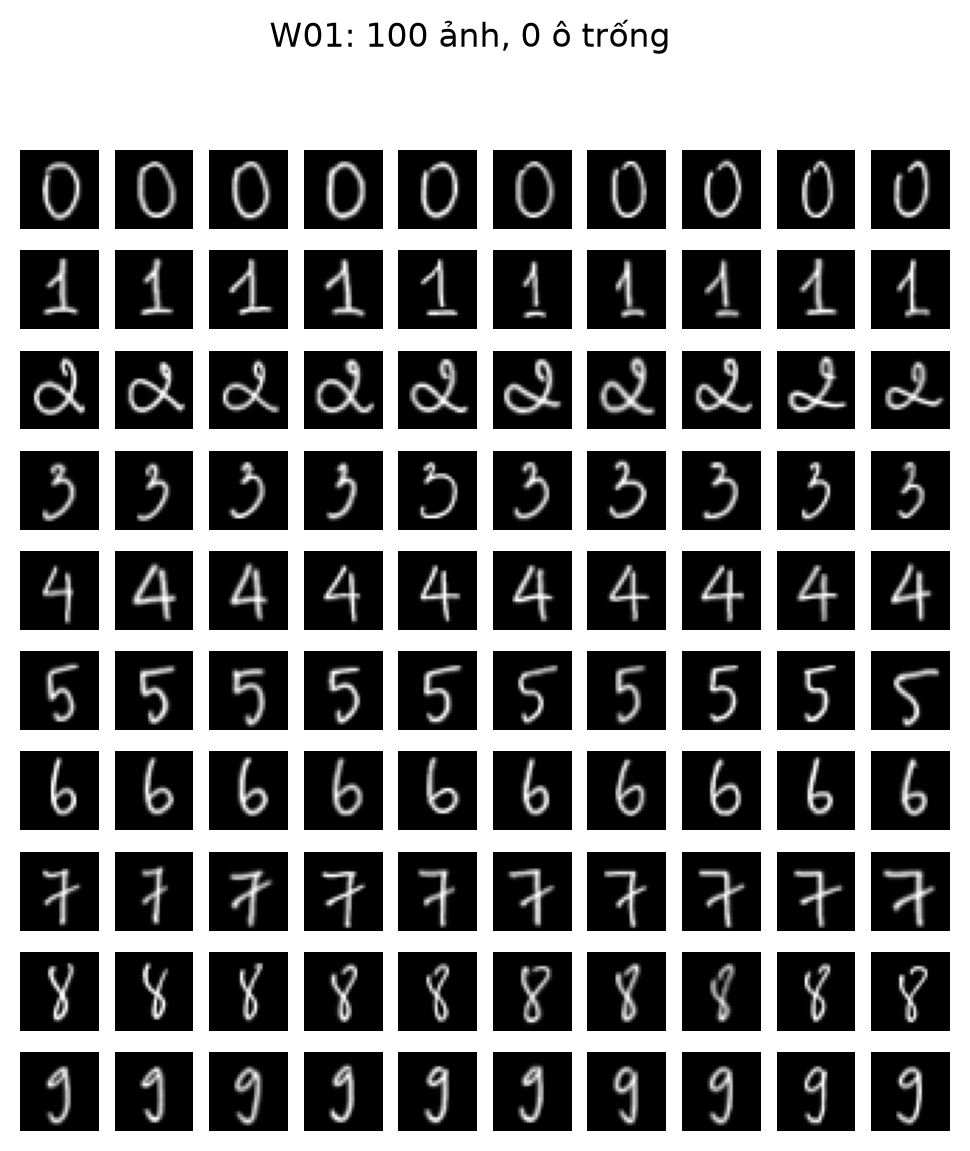
\includegraphics[width=\linewidth,trim=0 0 0 18,clip]{figures/vn_cells_W01.png}
    \subcaption{100 ô của phiếu W01}
  \end{minipage}\hfill
  \begin{minipage}[c]{0.7\linewidth}\centering
    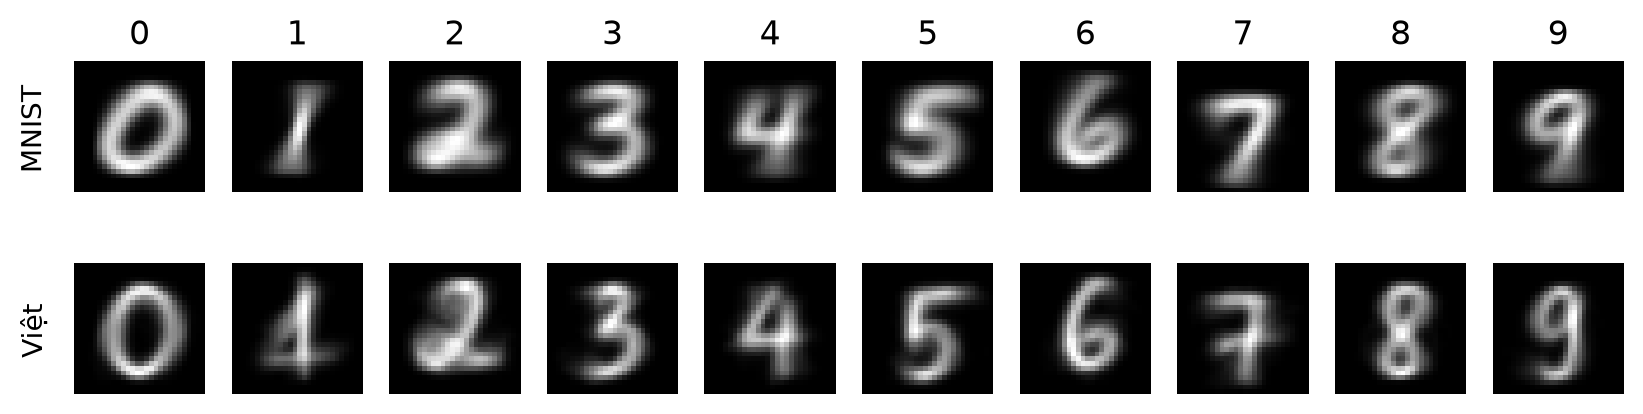
\includegraphics[width=\linewidth]{figures/vn_mean_images.png}
    \subcaption{Ảnh trung bình: MNIST (trên) và tập Việt (dưới)}
  \end{minipage}
  \caption{Tập chữ số người Việt sau khi xử lý. Ở ảnh trung bình, số 1 của người Việt có nét móc ở đầu và gạch chân, số 7 có gạch ngang ở giữa, và các chữ số nói chung đứng thẳng hơn MNIST.}
  \label{fig:vndata}
\end{figure}

\subsection{Datasheet}
Bảng~\ref{tab:datasheet} tóm tắt tập dữ liệu theo khung \emph{Datasheets for Datasets} %\cite{gebru2021}.

\begin{table}[H]
\centering
\caption{Datasheet của tập chữ số viết tay người Việt.}
\label{tab:datasheet}
\small
\begin{tabularx}{\linewidth}{@{}p{2.9cm}X@{}}
\toprule
Mục đích & Đo mức lệch miền giữa MNIST và chữ số người Việt; đánh giá augmentation và việc bổ sung ít dữ liệu đúng miền. \\
Thành phần & 2.980 ảnh xám $28\times28$, nhãn 0--9, mã người viết W01--W30; 294--300 ảnh/lớp, khoảng 100 ảnh/người. \\
Thu thập & Phiếu in A4 lưới $10\times10$ có 4 ô đen định vị; viết bằng bút bi và bút nước, chụp bằng điện thoại trong \todo{điều kiện ánh sáng}; thời gian \todo{tháng/năm}. \\
Tiền xử lý & Như Hình~\ref{fig:vnpipe}; 0 ô trống, loại thủ công 20 ô lỗi. Ảnh phiếu gốc được giữ riêng, không công bố. \\
Đồng ý \& riêng tư & Người viết ký xác nhận trên phiếu; dữ liệu công bố không chứa tên hay chữ ký, chỉ có mã người viết. \\
Hạn chế & 30 người viết nên chưa đại diện cho người Việt nói chung; mỗi người viết 10 lần liên tiếp nên các ảnh của cùng một người rất giống nhau. \\
Sử dụng & Chỉ dùng cho mục đích học tập trong môn học; không dùng để nhận diện người viết. \\
\bottomrule
\end{tabularx}
\end{table}

\subsubsection{Thiết kế thí nghiệm}
Bảng~\ref{tab:vnexp} mô tả ba thí nghiệm. Cả bốn bộ phân lớp dùng nguyên cấu hình đã chọn trên validation MNIST (Na\"{\i}ve Bayes $\alpha=0{,}001$; Logistic Regression $\eta=0{,}1$; MLP $(784,256,128,10)$; Random Forest 50 cây, độ sâu tối đa 15), \emph{không} chỉnh lại theo tập Việt.

\begin{table}[H]
\centering
\caption{Ba thí nghiệm về lệch miền.}
\label{tab:vnexp}
\small
\begin{tabularx}{\linewidth}{@{}lp{3.6cm}p{3.1cm}X@{}}
\toprule
& Huấn luyện trên & Kiểm tra trên & Câu hỏi \\
\midrule
(a) & MNIST & Người Việt & Lệch miền làm giảm bao nhiêu? Lớp nào, mô hình nào chịu ảnh hưởng nhất? \\
(b) & MNIST + augmentation & Người Việt & Dạy mô hình ``chịu'' xoay, dịch, nhiễu có giảm được lệch miền không? \\
(c) & MNIST + \emph{một phần} người Việt & \emph{Những người Việt còn lại} & Thêm một ít dữ liệu đúng miền giúp được bao nhiêu? \\
\bottomrule
\end{tabularx}
\end{table}

Tập Việt được chia \emph{theo người viết} (\code{writer\_split}, 30\% người viết làm tập kiểm tra): toàn bộ ảnh của một người chỉ nằm ở một phía. Nếu chia ngẫu nhiên theo ảnh, mô hình sẽ được kiểm tra trên chính nét chữ đã thấy khi huấn luyện và kết quả sẽ lạc quan giả tạo. Cả ba thí nghiệm được đánh giá trên \emph{cùng} nhóm người viết kiểm tra; việc chia được lặp với 3 hạt giống và báo cáo trung bình $\pm$ độ lệch chuẩn. Ở (b), mỗi ảnh MNIST được bổ sung một bản biến đổi ngẫu nhiên (xoay, dịch, nhiễu; \todo{tham số trong \code{augment\_dataset}}), tập huấn luyện tăng lên 108.000 ảnh. Ở (c), ảnh của những người viết thuộc phần huấn luyện được lặp lại 5 lần rồi ghép vào 54.000 ảnh MNIST, để vài nghìn ảnh Việt không bị lấn át.


\subsection{Tăng cường dữ liệu và thí nghiệm độ bền}

\subsubsection{Ý tưởng và cách cài đặt}

Tăng cường dữ liệu (\textit{Data Augmentation}) tạo thêm các biến đổi từ ảnh huấn luyện, giúp mô hình nhận dạng chữ số tốt
hơn khi hình ảnh bị thay đổi. Thí nghiệm độ bền (\textit{Robustness})
đánh giá khả năng duy trì độ chính xác khi ảnh đầu vào bị xoay,
dịch chuyển hoặc thêm nhiễu.

Hàm \texttt{augment\_dataset()} tạo thêm một bản biến đổi cho mỗi
ảnh huấn luyện (\texttt{copies=1}). Dữ liệu gốc và dữ liệu mới được
ghép lại, đồng thời giữ nguyên nhãn:
\[
X_{\mathrm{aug}}=[X_{\mathrm{tr}};X_{\mathrm{trans}}],
\qquad
y_{\mathrm{aug}}=[y_{\mathrm{tr}};y_{\mathrm{tr}}].
\]

Hàm \texttt{perturb()} tạo dữ liệu kiểm tra biến đổi theo ba phép:
xoay ảnh ở các góc $0^\circ,10^\circ,20^\circ,30^\circ,45^\circ$;
dịch ảnh chéo xuống-phải từ $0$ đến $4$ pixel; và thêm nhiễu
Gaussian với $\sigma\in\{0,0.1,0.2,0.3,0.5\}$.
Các mô hình được huấn luyện trên dữ liệu gốc và dữ liệu tăng cường,
sau đó đánh giá trên cùng tập kiểm tra đã biến đổi.

Độ chính xác được tính theo:
\[
\mathrm{Accuracy}=
\frac{1}{N}\sum_{i=1}^{N}
\mathbf{1}(\hat{y}_i=y_i),
\]
trong đó $N$ là số ảnh kiểm tra, $\hat{y}_i$ là nhãn dự đoán và
$y_i$ là nhãn thực tế.

\subsubsection{Kết quả thực nghiệm}

\begin{figure}[htbp]
    \centering

    % Bảng ở trên
    \begin{minipage}{\textwidth}
        \centering
        \captionof{table}{So sánh độ chính xác của các mô hình trên ảnh gốc,
ảnh xoay $30^\circ$ và ảnh dịch chuyển $3$ pixel (\%)}
        \label{tab:robustness}
        \small
        \begin{tabular}{lccc}
            \hline
            \textbf{Mô hình} &
            \textbf{Ảnh gốc} &
            \textbf{Xoay $30^\circ$} &
            \textbf{Dịch 3 pixel} \\
            \hline
            Logistic Regression       & 92.13 & 55.83 & 11.17 \\
            Logistic Regression + aug & 91.24 & 55.62 & 23.13 \\
            MLP                       & 98.09 & 78.44 & 20.19 \\
            MLP + aug                 & 98.58 & 86.88 & 77.91 \\
            Multinomial NB            & 83.64 & 44.75 & 16.72 \\
            Multinomial NB + aug      & 81.06 & 43.99 & 9.53 \\
            Random Forest             & 96.45 & 71.29 & 16.05 \\
            Random Forest + aug       & 96.18 & 77.49 & 37.39 \\
            \hline
        \end{tabular}
    \end{minipage}

    \vspace{0.5cm}

    % Hình ở dưới
    \begin{minipage}{\textwidth}
        \centering
        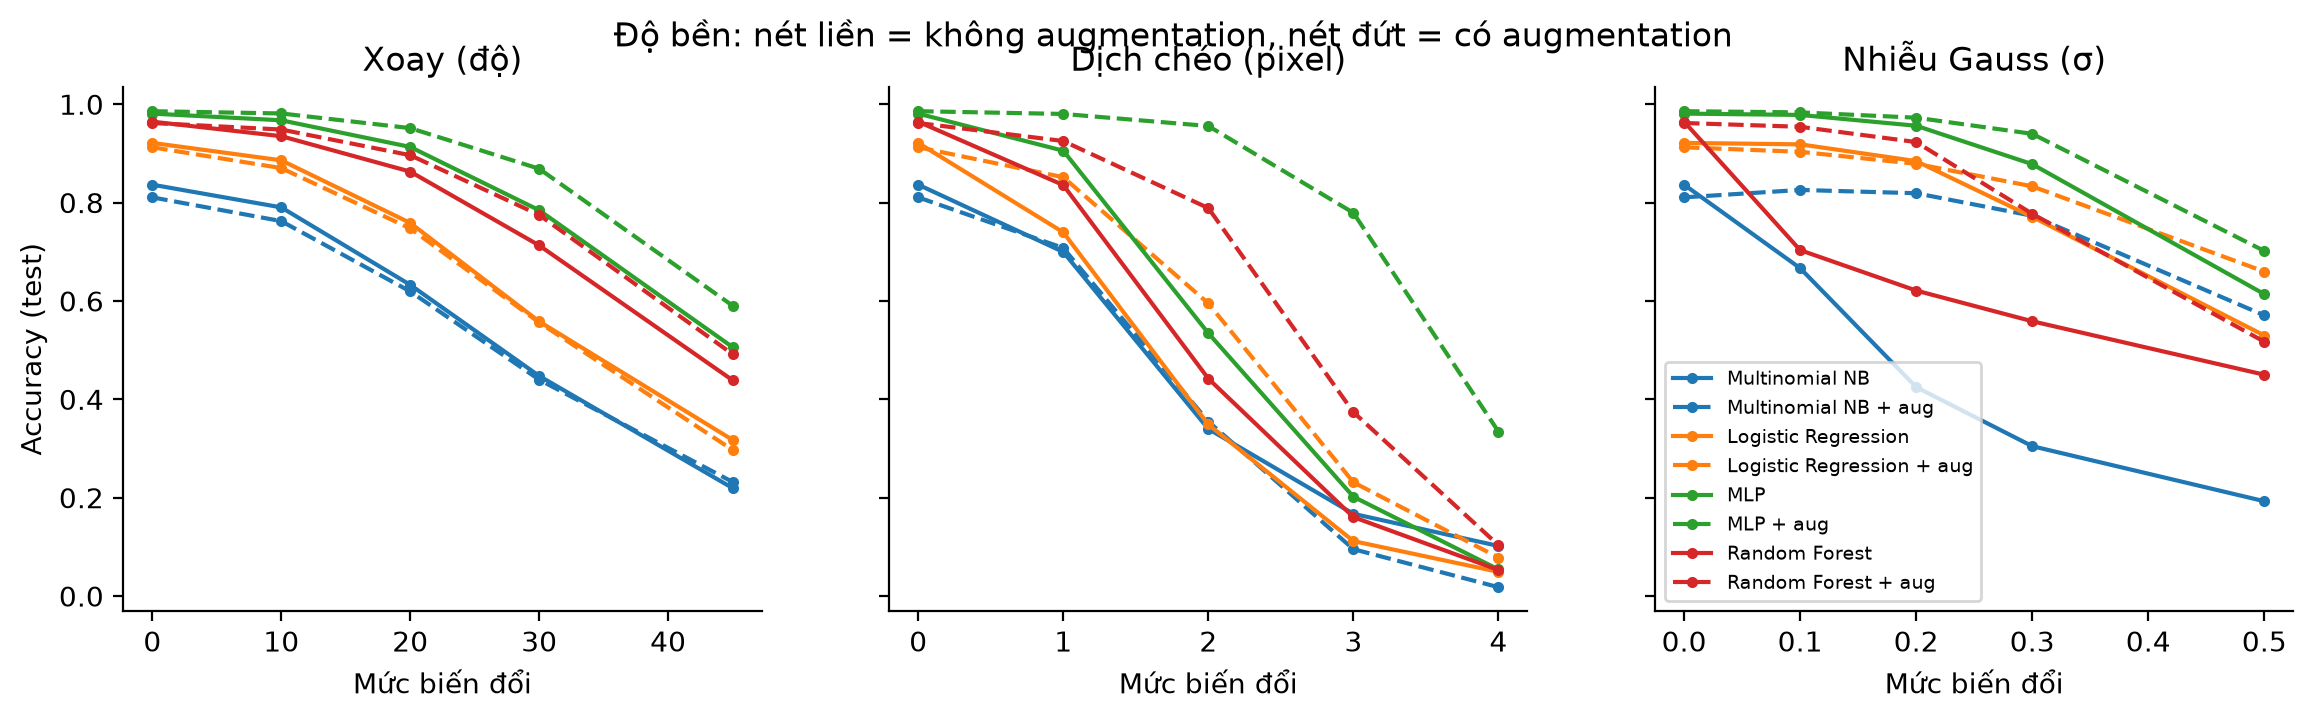
\includegraphics[width=0.9\textwidth]
        {figures/robustness_test.png}
        \caption{Sự thay đổi độ chính xác của các mô hình theo mức độ biến đổi ảnh}
        \label{fig:robustness}
    \end{minipage}
\end{figure}

\subsubsection{Nhận xét}

Kết quả cho thấy tăng cường dữ liệu cải thiện độ bền của một số
mô hình. Với phép xoay $30^\circ$, MLP có augmentation đạt
$86.88\%$, cao hơn mức $78.44\%$ của mô hình thông thường.
Khi dịch ảnh $3$ pixel, độ chính xác tăng từ $20.19\%$ lên
$77.91\%$. Random Forest cũng cải thiện ở cả hai phép biến đổi.

Ngược lại, Logistic Regression gần như không cải thiện khi xoay
ảnh, còn Multinomial Naive Bayes giảm độ chính xác sau augmentation.
Như vậy, hiệu quả của tăng cường dữ liệu phụ thuộc vào mô hình
và loại biến đổi, không phải lúc nào cũng mang lại kết quả tốt hơn.

Thí nghiệm này đánh giá độ bền trên ảnh MNIST bị biến đổi, chưa
đánh giá trực tiếp khả năng nhận dạng chữ số viết tay của người Việt.


\subsection{Giao diện demo vẽ và nhận diện chữ số}

\subsubsection{Mục đích}

Giao diện demo được xây dựng bằng thư viện Gradio, cho phép
người dùng vẽ trực tiếp chữ số viết tay từ 0 đến 9 và quan sát
kết quả nhận dạng. Hệ thống sử dụng bốn mô hình đã huấn luyện
gồm Multinomial Naive Bayes, Logistic Regression, MLP và
Random Forest. Các mô hình được lưu dưới dạng \texttt{.pkl}
trong thư mục \texttt{results/models/} và được tải khi khởi
chạy ứng dụng.

\subsubsection{Giao diện và chức năng}

Hình~\ref{fig:digit-demo-interface} minh họa giao diện demo
nhận diện chữ số viết tay. Các chức năng chính bao gồm:

\begin{itemize}
    \item \textbf{Vẽ chữ số:} Người dùng vẽ trực tiếp chữ số
    trên vùng vẽ của ứng dụng.

    \item \textbf{Tiền xử lý ảnh:} Ảnh đầu vào được chuyển
    sang mức xám, làm sạch và chuẩn hóa về kích thước
    $28\times28$ pixel.

    \item \textbf{Dự đoán:} Ảnh sau tiền xử lý được chuyển
    thành vector gồm 784 đặc trưng để đưa vào bốn mô hình.

    \item \textbf{Hiển thị kết quả:} Giao diện hiển thị các
    chữ số có xác suất dự đoán cao nhất của từng mô hình.

    \item \textbf{So sánh mô hình:} Hệ thống hiển thị thời gian
    dự đoán và thông báo khi các mô hình đồng thuận hoặc
    bất đồng về kết quả nhận dạng.
\end{itemize}

\begin{figure}[H]
    \centering
    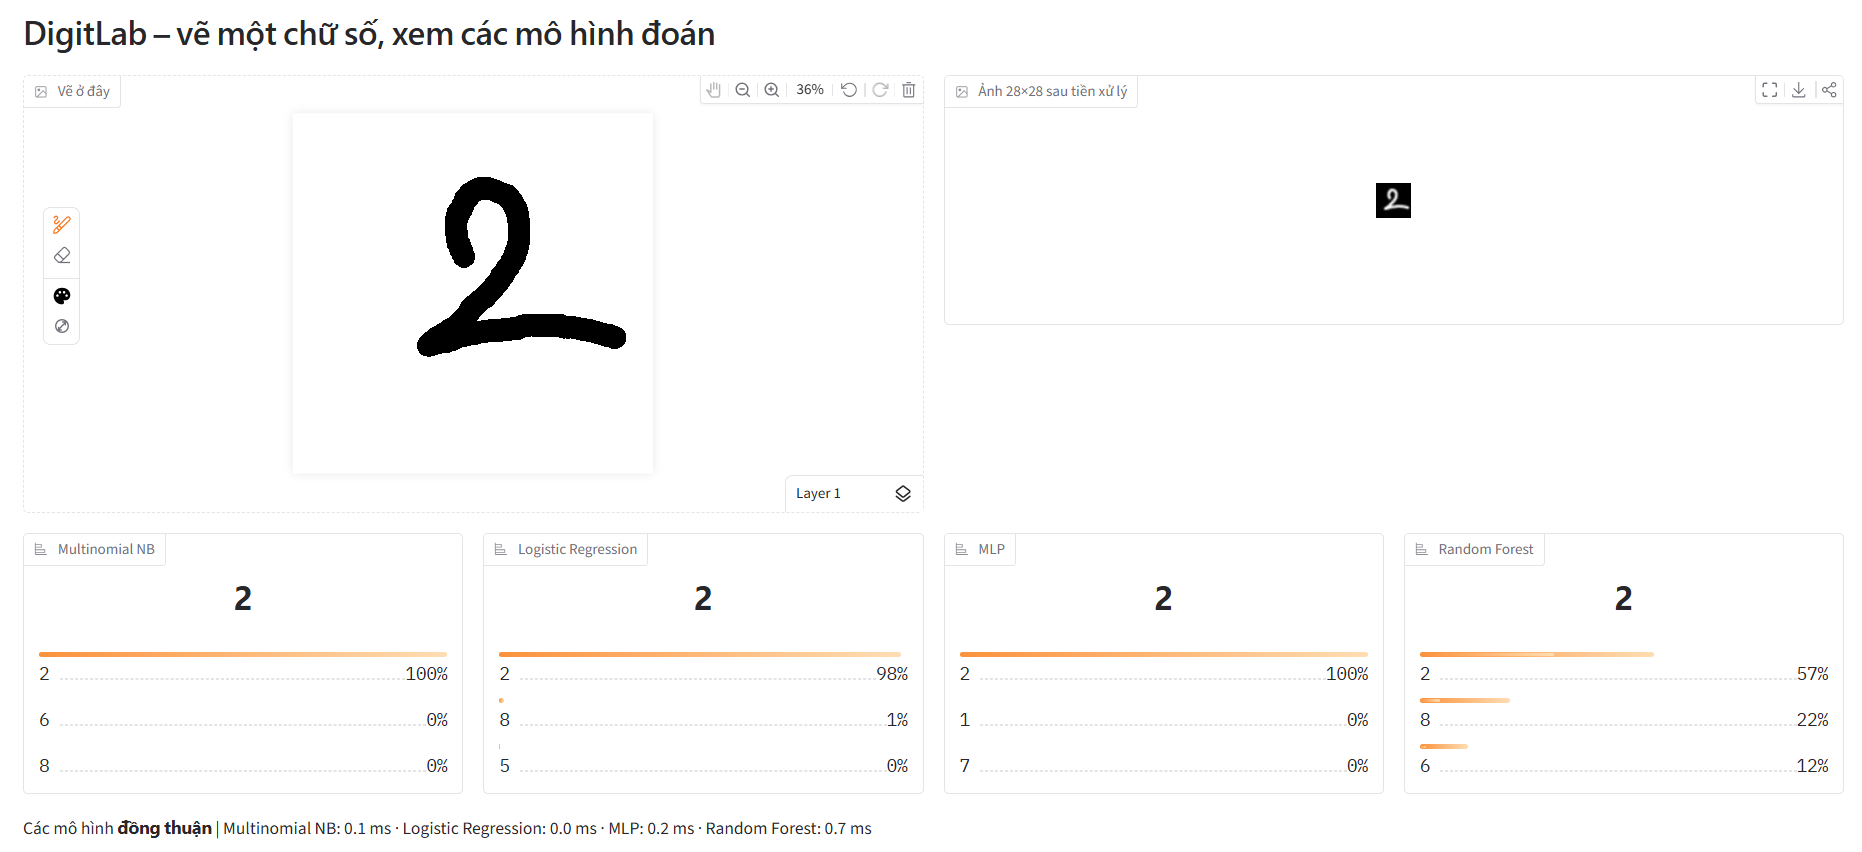
\includegraphics[
        width=0.82\textwidth,
        height=0.42\textheight,
        keepaspectratio
    ]{figures/digit_demo_interface.png}
    \caption{Giao diện demo nhận diện chữ số viết tay.}
    \label{fig:digit-demo-interface}
\end{figure}

\subsubsection{Quy trình nhận dạng}

Quy trình nhận dạng gồm hai phần: chuẩn bị mô hình đã huấn
luyện và xử lý ảnh đầu vào của người dùng. Các mô hình được
huấn luyện trong \texttt{main.ipynb}, lưu thành các tệp
\texttt{.pkl} và được tải trong \texttt{app.py}. Khi người
dùng vẽ chữ số, chương trình lần lượt thực hiện chuyển ảnh
sang mức xám, làm sạch, chuẩn hóa kích thước và chuyển ảnh
thành vector đặc trưng trước khi dự đoán.

Hình~\ref{fig:digit-demo-diagram} trình bày sơ đồ tổng quát
của quy trình này.

\begin{figure}[H]
    \centering
    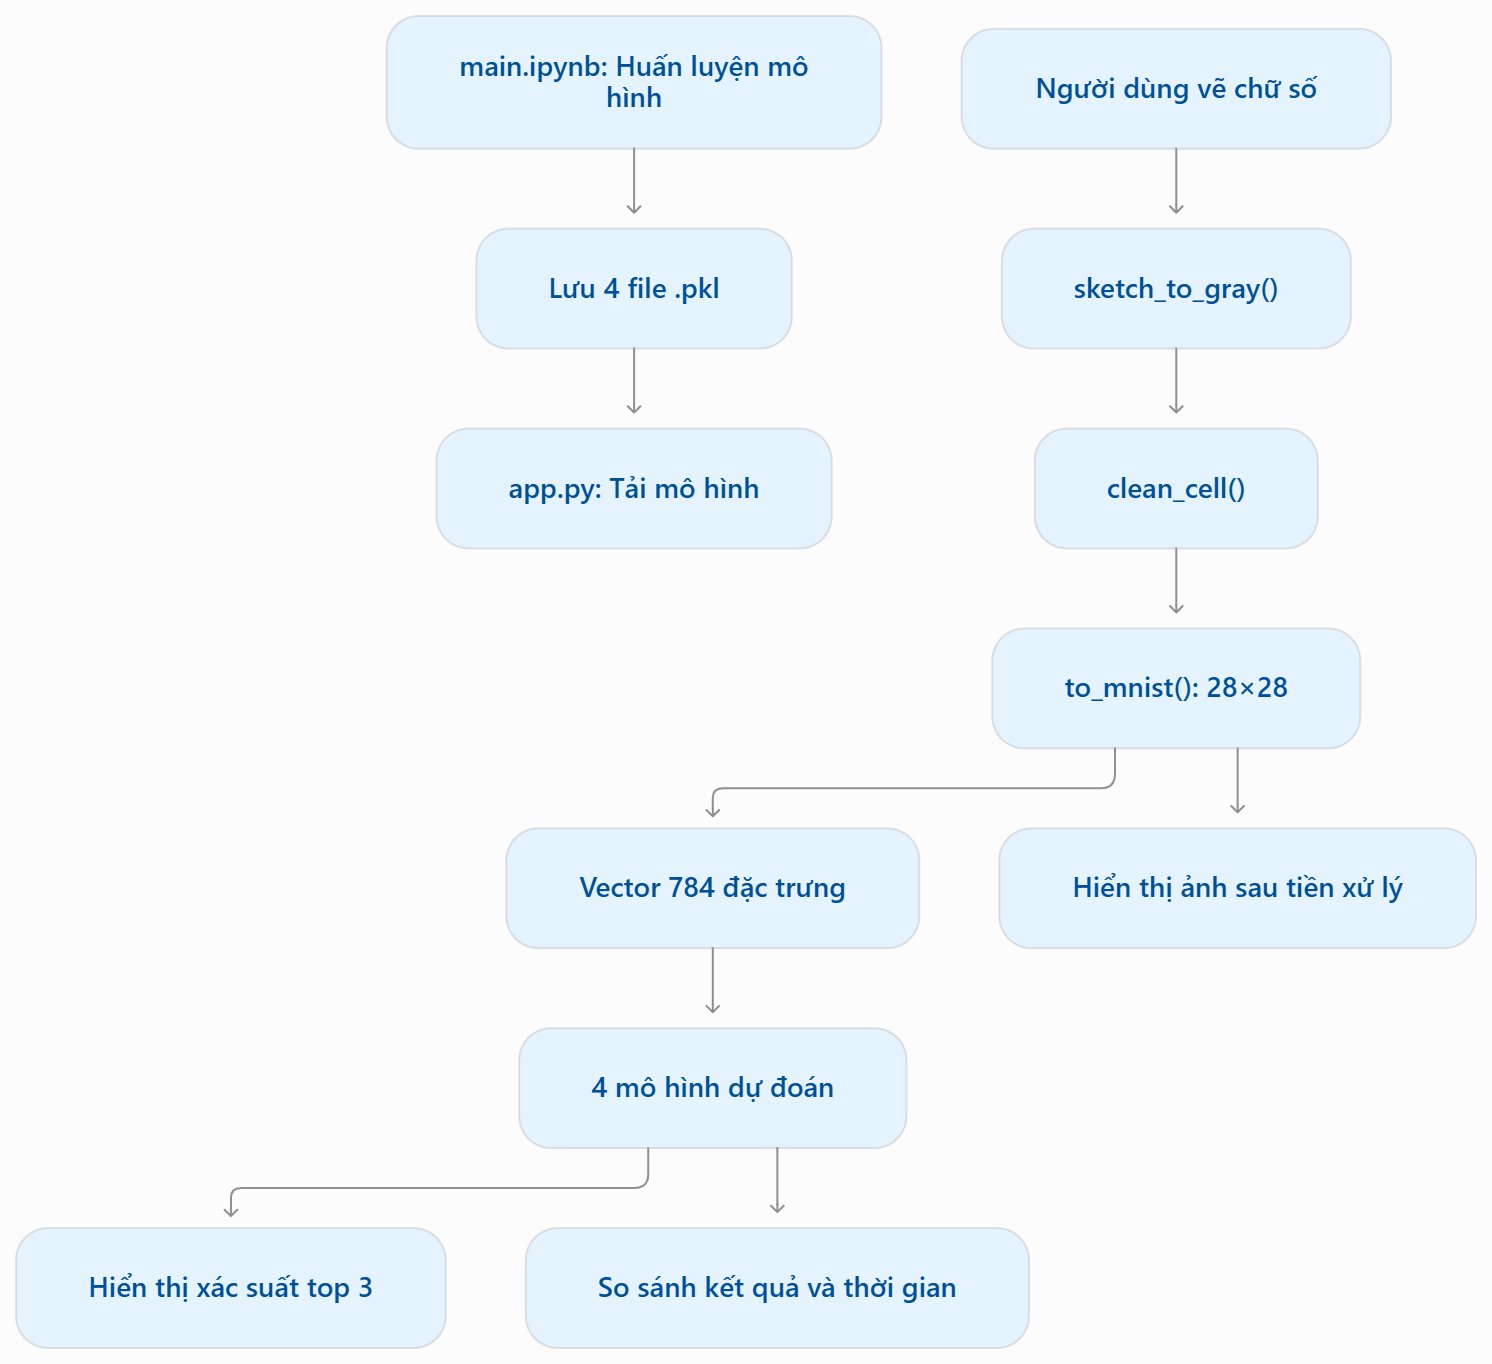
\includegraphics[
        width=0.88\textwidth,
        height=0.48\textheight,
        keepaspectratio
    ]{figures/digit_demo_diagram.png}
    \caption{Sơ đồ quy trình hoạt động của chương trình demo.}
    \label{fig:digit-demo-diagram}
\end{figure}

\subsubsection{Kiểm thử và minh họa kết quả}

Ngoài giao diện Gradio, quy trình nhận dạng còn được kiểm
thử trong \texttt{main.ipynb}. Chương trình tạo ảnh chữ số
minh họa, thực hiện tiền xử lý và đưa ảnh vào các mô hình
để quan sát kết quả dự đoán.

\begin{figure}[H]
    \centering
    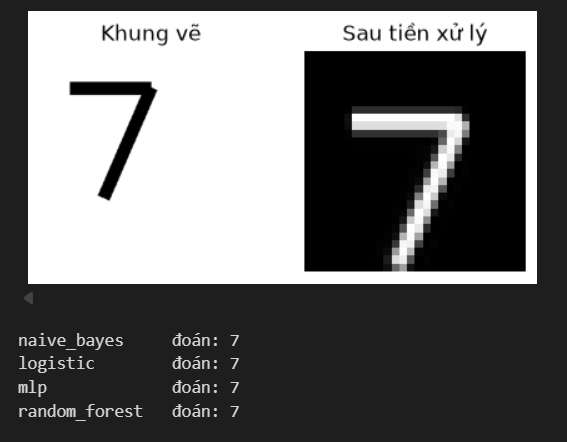
\includegraphics[
        width=0.78\textwidth,
        height=0.36\textheight,
        keepaspectratio
    ]{figures/digit_demo_inMain.png}
    \caption{Kiểm thử quy trình nhận dạng trong \texttt{main.ipynb}.}
    \label{fig:digit-demo-inmain}
\end{figure}

Để minh họa sự khác biệt giữa kết quả dự đoán của các mô
hình, Hình~\ref{fig:digit-demo-right} trình bày trường hợp
các mô hình đồng thuận, trong khi
Hình~\ref{fig:digit-demo-wrong} trình bày trường hợp các
mô hình đưa ra dự đoán khác nhau.

\begin{figure}[H]
    \centering
    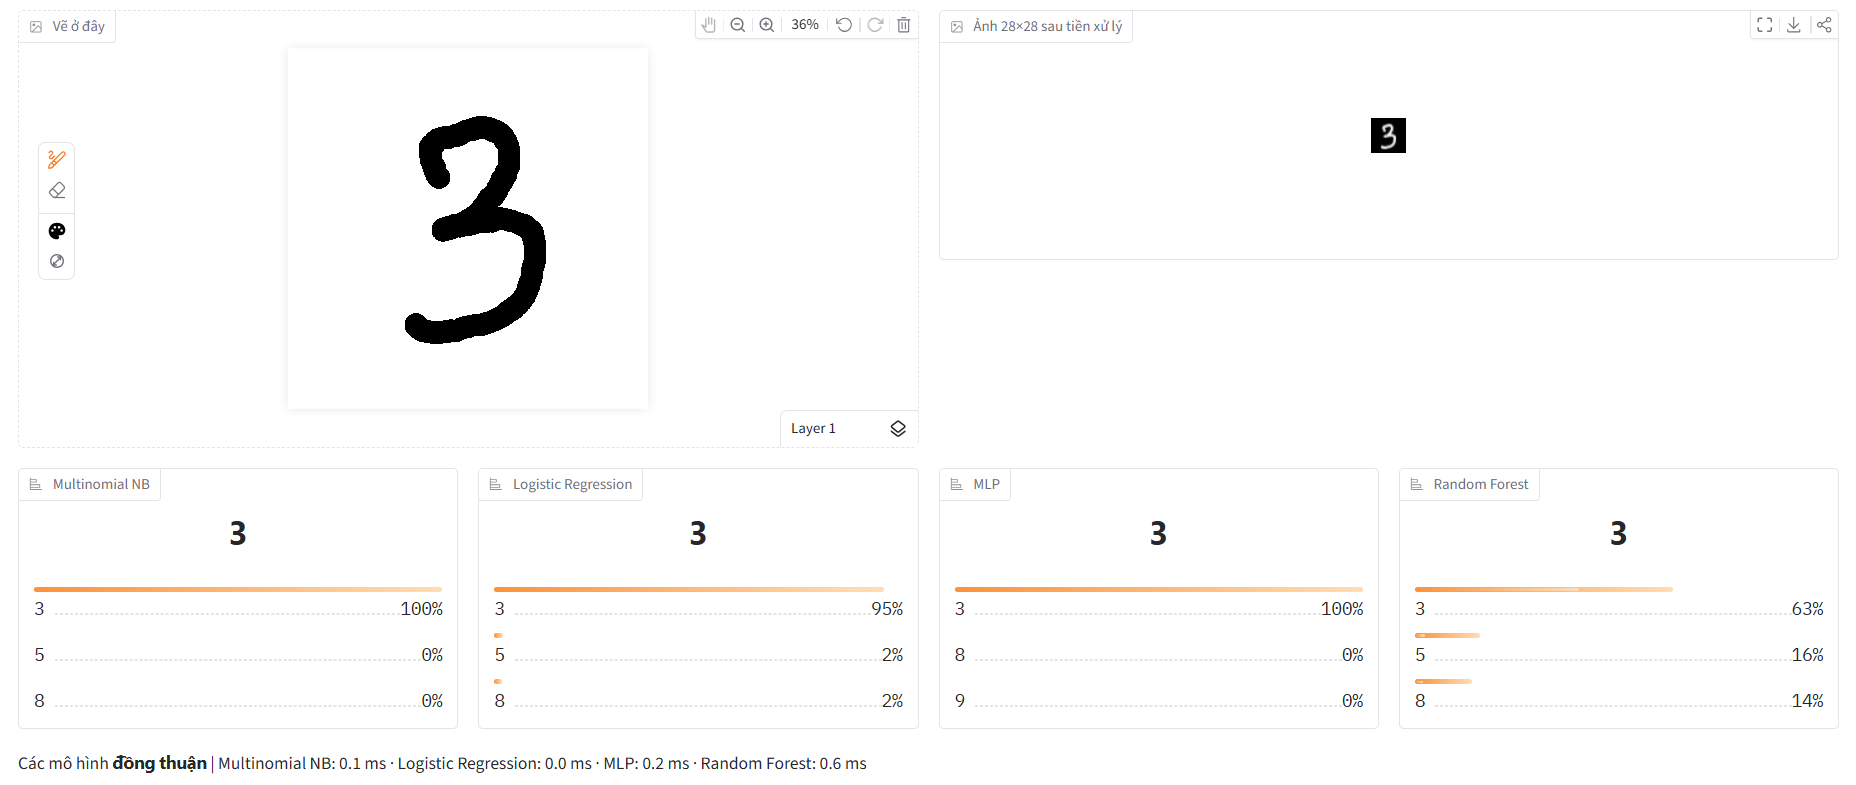
\includegraphics[
        width=0.78\textwidth,
        height=0.34\textheight,
        keepaspectratio
    ]{figures/digit_demo_right.png}
    \caption{Trường hợp các mô hình đồng thuận về kết quả dự đoán.}
    \label{fig:digit-demo-right}
\end{figure}

\begin{figure}[H]
    \centering
    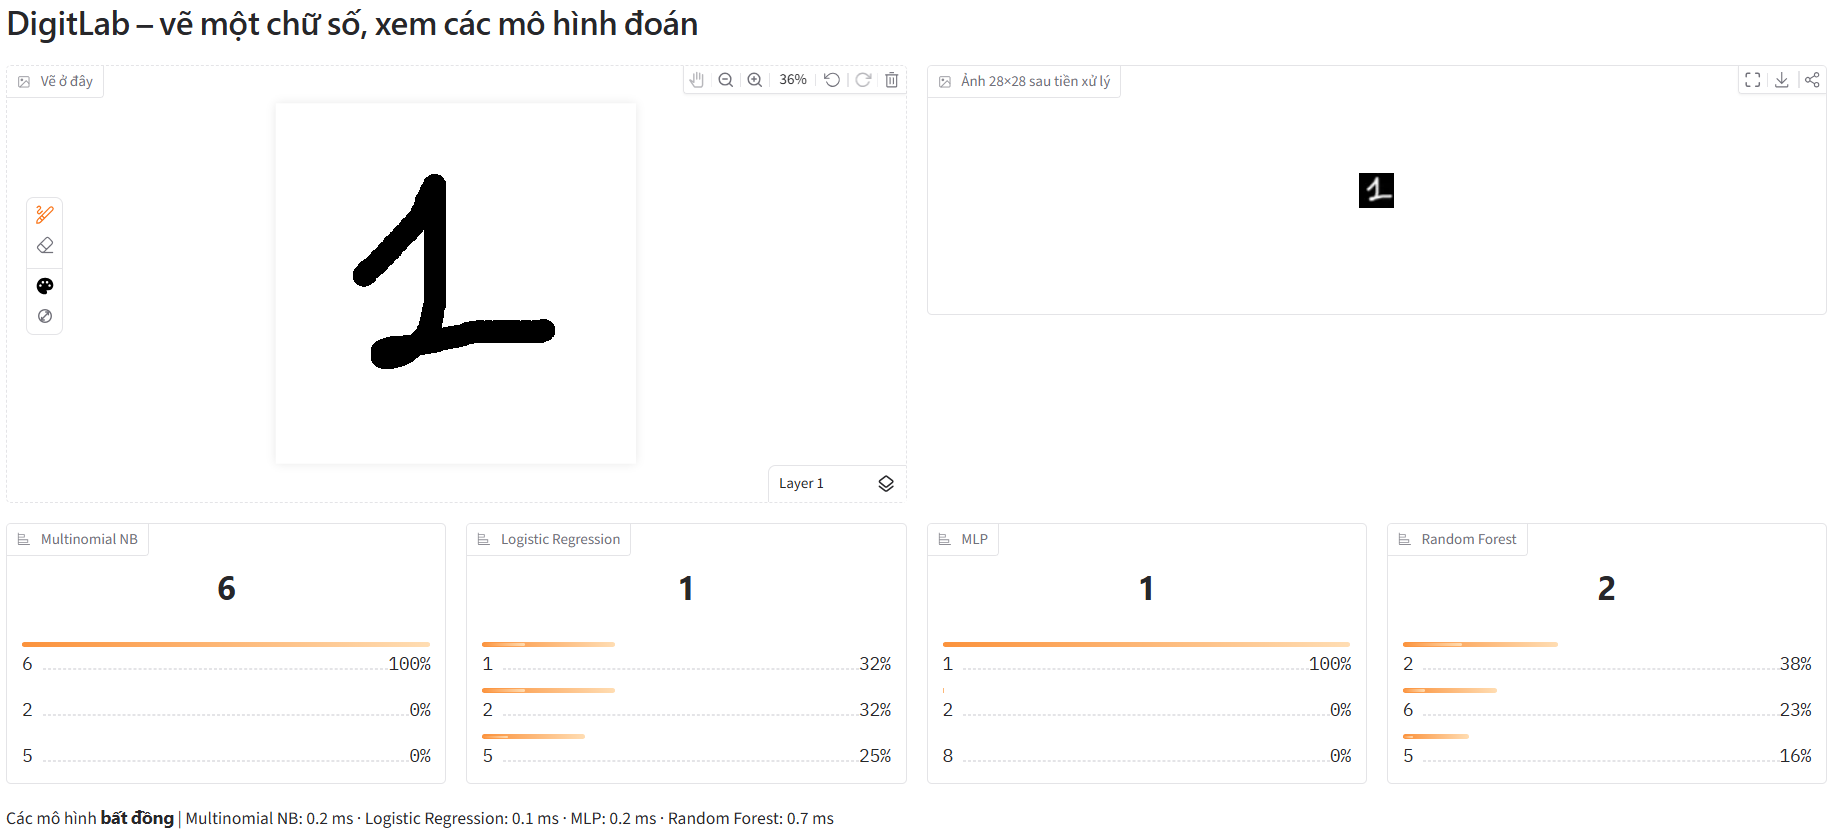
\includegraphics[
        width=0.78\textwidth,
        height=0.34\textheight,
        keepaspectratio
    ]{figures/digit_demo_wrong.png}
    \caption{Trường hợp các mô hình bất đồng về kết quả dự đoán.}
    \label{fig:digit-demo-wrong}
\end{figure}

\subsubsection{Đánh giá}

Giao diện demo giúp trực quan hóa quá trình nhận diện chữ số
viết tay, đồng thời hỗ trợ so sánh kết quả dự đoán và thời
gian suy luận của bốn mô hình. Tuy nhiên, việc các mô hình
đồng thuận không đồng nghĩa với dự đoán chính xác. Để xác
định trường hợp nhận dạng đúng hoặc sai, cần đối chiếu kết
quả dự đoán với nhãn thực tế của ảnh đầu vào. Các hình ảnh
minh họa chủ yếu phục vụ kiểm thử chức năng, không thay thế
cho việc đánh giá định lượng trên tập dữ liệu độc lập.


\section{Kết luận và hướng phát triển}

\subsection{Tóm tắt quá trình thực hiện}

Đề tài được thực hiện qua các bước: chuẩn bị và tiền xử lý
dữ liệu MNIST cùng dữ liệu chữ viết tay người Việt được nhóm thu thập; xây dựng,
huấn luyện và đánh giá bốn mô hình Multinomial Naive Bayes,
Logistic Regression, MLP và Random Forest; thử nghiệm bổ sung
dữ liệu đúng miền và tăng cường dữ liệu; cuối cùng xây dựng
giao diện demo bằng Gradio để trực quan hóa kết quả dự đoán
và so sánh thời gian xử lý giữa các mô hình.

\subsection{Kết luận}

Trong bốn mô hình được thử nghiệm, MLP đạt kết quả tốt nhất
trên tập kiểm thử MNIST với accuracy $98.09\%$. Khi áp dụng
trên chữ viết tay người Việt, accuracy của MLP giảm từ
$98.13\%$ xuống $89.35\%$. Việc bổ sung dữ liệu đúng miền
giúp accuracy tăng lên $94.56\%$ đối với MLP và từ $68.78\%$
lên $87.89\%$ đối với Random Forest.

Ngoài ra, tăng cường dữ liệu giúp MLP đạt accuracy $77.91\%$
khi ảnh bị dịch $3$ pixel, cao hơn đáng kể so với $20.19\%$
của mô hình không tăng cường dữ liệu.

\subsection{Hướng phát triển}

Trong tương lai, nhóm sẽ thử nghiệm mô hình CNN để khai
thác đặc trưng không gian của ảnh tốt hơn, đồng thời thu thập
thêm dữ liệu chữ viết tay tiếng Việt đa dạng về người viết
và kiểu chữ nhằm cải thiện khả năng tổng quát hóa của mô hình.


% References
\cleardoublepage
\phantomsection
\addcontentsline{toc}{section}{Tài liệu tham khảo}
\nocite{*}
\bibliographystyle{plain}
\bibliography{ref/ref}

% Appendix
\appendix
% Add \cleardoublepage to move appendices to next page.

\section{Phân công công việc và khai báo sử dụng AI}

\subsection{Bảng phân công công việc và tỷ lệ đóng góp}

Bảng dưới đây trình bày nhiệm vụ được phân công và tỷ lệ
đóng góp của từng thành viên trong quá trình thực hiện đề tài.

\begin{table}[htbp]
    \centering
    \small
    \renewcommand{\arraystretch}{1.3}
    \begin{tabular}{
        |>{\centering\arraybackslash}p{0.8cm}
        |p{3cm}
        |p{7cm}
        |>{\centering\arraybackslash}p{2cm}|
    }
        \hline
        \textbf{STT} &
        \textbf{Thành viên} &
        \textbf{Công việc thực hiện} &
        \textbf{Đóng góp (\%)} \\
        \hline
        1 & Nguyễn Thị Huệ Giang & Xây dựng phương pháp Multinomial NB, Random Forest, thu thập và xử lý phiếu chữ viết tay & 100\% \\
        \hline
        2 & Lâm Hà Quỳnh Như & Tải, tiền xử lý, chia tập dữ liệu, xây dựng phương pháp MLP, thu thập và xử lý phiếu chữ viết tay& 100\% \\
        \hline
        3 & Hồ Việt Thuận Phú & Logistic Regression, thí nghiệm độ bền (augmentation),tạo tập dữ liệu Việt, xây dựng khung demo, thực hiện các đánh giá & 100\% \\
        \hline
        \multicolumn{3}{|r|}{\textbf{Tổng cộng}} &
        \textbf{100\%} \\
        \hline
    \end{tabular}
    \caption{Phân công công việc và tỷ lệ đóng góp của các thành viên.}
    \label{tab:phan-cong}
\end{table}

\subsection{Khai báo sử dụng trí tuệ nhân tạo (AI)}

Trong quá trình thực hiện đề tài, nhóm có sử dụng công cụ
trí tuệ nhân tạo (AI) để hỗ trợ giải thích thuật toán, tham
khảo cách triển khai chương trình, phát hiện và sửa lỗi
mã nguồn, cũng như chỉnh sửa nội dung báo cáo.

Các kết quả do AI đề xuất được nhóm xem xét, kiểm tra và
điều chỉnh trước khi sử dụng. Nhóm chịu trách nhiệm về
tính chính xác của nội dung, mã nguồn và kết quả thực nghiệm
được trình bày trong báo cáo.

\begin{table}[htbp]
    \centering
    \small
    \renewcommand{\arraystretch}{1.3}
    \begin{tabular}{
        |p{3.5cm}
        |p{5cm}
        |p{5cm}|
    }
        \hline
        \textbf{Công cụ AI} &
        \textbf{Mục đích sử dụng} &
        \textbf{Phạm vi sử dụng} \\
        \hline
        ChatGPT &
        Hỗ trợ giải thích, gợi ý mã nguồn và sửa lỗi báo cáo&
        Tham khảo trong quá trình viết báo cáo \\
        \hline
        Claude &
        \textbullet~Soạn tài liệu hướng dẫn: kiến thức nền, công thức, ví dụ tính tay \newline
        \textbullet~Gợi ý mã nguồn khung: \texttt{metrics.py}, \texttt{vn\_digits.py}, \texttt{experiments.py}, \texttt{app.py}, notebook \texttt{main.ipynb} \newline
        \textbullet~Thiết kế phiếu thu thập chữ số viết tay \newline
        \textbullet~Giải thích và sửa lỗi khi chạy \newline &
        \textbullet~Giải thích thuật toán và cách kiểm chứng (gradient check, đối chiếu scikit-learn) \newline
        \textbullet~Rà soát code nhóm tự viết \newline \\
        \hline
    \end{tabular}
    \caption{Khai báo công cụ AI được sử dụng trong đề tài.}
    \label{tab:khai-bao-ai}
\end{table}



\end{document}